%
% (c) 2011-2016 - Eric NOULARD  <eric.noulard@gmail.com>
% This is a CMake (https://cmake.org) tutorial
% the material is open and may be found on github:
% https://github.com/TheErk/CMake-tutorial
%
% This set of slides are licensed with
% the creative commons CC-BY-SA license.
%
% For printed version uncomment trans
% If you want nice PDF presentation
% you may use Impress!ve: http://impressive.sourceforge.net/
% you use https://github.com/jberger/MakeBeamerInfo in order
% to create the impress!ve script more easily
%
\documentclass[compress,slidestop,table,usepdftitle=false
%               trans
              ]
               {beamer}

\usepackage{iwona}
\usepackage[english]{babel}
\usepackage[utf8]{inputenc}
\usepackage{xcolor}
\definecolor{cmakeblue}{RGB}{84,84,216}
\definecolor{cmakered}{RGB}{235,69,69}
\definecolor{cmakegreen}{RGB}{0,219,0}
\colorlet{cmaketimec}{green}
\colorlet{buildtimec}{red}
\colorlet{installtimec}{black}
\colorlet{cpacktimec}{blue}

\usepackage{graphicx}
\graphicspath{{figures/}{images/}}
\DeclareGraphicsExtensions{.eps,.png,.pdf,.eps,.jpg}

% Uncomment this for handout mode
\mode<handout>{
    \usepackage{pgfpages}
    \pgfpagesuselayout{2 on 1}[a4paper,border shrink=5mm]
    \setbeamercolor{background canvas}{bg=black!5}
}

\mode<presentation>{
     %\setbeamercovered{transparent}
     \setbeamercovered{invisible}
     % progressbar is a nice beamer theme by Sylvain BOUVERET
     % http://recherche.noiraudes.net/fr/LaTeX.php
     \usetheme{progressbar}
     \progressbaroptions{
               %headline=sections,
               imagename=figures/CMake-logo-triangle-small.png,
               titlepage=normal,
               frametitle=picture-section
                        }
}


\usepackage{fancyvrb}
\VerbatimFootnotes

\usepackage{ulem}
\usepackage{multirow}
\usepackage{multicol}
\usepackage{tikz}
\usetikzlibrary{arrows,shapes}
\usetikzlibrary{patterns,snakes,automata,topaths}
\usetikzlibrary{matrix,chains}
\usetikzlibrary{shadows}
\usetikzlibrary{positioning}
\usetikzlibrary{shadings}
\usetikzlibrary{calc}
\tikzstyle{na} = [baseline=-.5ex]
\tikzstyle{every picture}+=[remember picture]


%\usepackage[underline=true,rounded corners=false]{pgf-umlsd}

\usepackage[formats]{listings}
% define CMake script language (http://www.cmake.org)
\lstdefinelanguage{CMake}
	{
         % keywords are the CMake commands
         morekeywords={
add_custom_command,
add_custom_target,
add_definitions,
add_dependencies,
add_executable,
add_library,
add_subdirectory,
add_test,
aux_source_directory,
break,
build_command,
cmake_minimum_required,
cmake_policy,
configure_file,
create_test_sourcelist,
define_property,
else,
elseif,
enable_language,
enable_testing,
endforeach,
endfunction,
endif,
endmacro,
endwhile,
execute_process,
export,
file,
find_file,
find_library,
find_package,
find_path,
find_program,
fltk_wrap_ui,
foreach,
function,
get_cmake_property,
get_directory_property,
get_filename_component,
get_property,
get_source_file_property,
get_target_property,
get_test_property,
if,
include,
include_directories,
include_external_msproject,
include_regular_expression,
install,
link_directories,
list,
load_cache,
load_command,
macro,
mark_as_advanced,
math,
message,
option,
project,
qt_wrap_cpp,
qt_wrap_ui,
remove_definitions,
return,
separate_arguments,
set,
set_directory_properties,
set_property,
set_source_files_properties,
set_target_properties,
set_tests_properties,
site_name,
source_group,
string,
target_link_libraries,
try_compile,
try_run,
unset,
variable_watch,
while,
build_name,
exec_program,
export_library_dependencies,
install_files,
install_programs,
install_targets,
link_libraries,
make_directory,
output_required_files,
remove,
subdir_depends,
subdirs,
use_mangled_mesa,
utility_source,
variable_requires,
write_file,
READ, WRITE, APPEND, RENAME, DOWNLOAD, UPLOAD,
GLOB, GLOB_RECURSE, MAKE_DIRECTORY,
TO_CMAKE_PATH, TO_NATIVE_PATH,
LENGTH,GET,FIND, APPEND, INSERT, REMOVE_ITEM, REMOVE_AT, REMOVE_DUPLICATES, REVERSE, SORT,
STATUS, WARNING, LOG, SHOW_PROGRESS, EXISTS, COMMAND,
RESULT_VARIABLE, OUTPUT_VARIABLE, ERROR_VARIABLE,
PROPERTIES
         },
         % CMake variables
         morekeywords=[2]{
<PROJECT-NAME>_BINARY_DIR,
<PROJECT-NAME>_SOURCE_DIR,
<PROJECT-NAME>_VERSION,
<PROJECT-NAME>_VERSION_MAJOR,
<PROJECT-NAME>_VERSION_MINOR,
<PROJECT-NAME>_VERSION_PATCH,
<PROJECT-NAME>_VERSION_TWEAK,
APPLE,
BORLAND,
BUILD_SHARED_LIBS,
CMAKE_<CONFIG>_POSTFIX,
CMAKE_<LANG>_ARCHIVE_APPEND,
CMAKE_<LANG>_ARCHIVE_CREATE,
CMAKE_<LANG>_ARCHIVE_FINISH,
CMAKE_<LANG>_CLANG_TIDY,
CMAKE_<LANG>_COMPILER,
CMAKE_<LANG>_COMPILER_ABI,
CMAKE_<LANG>_COMPILER_EXTERNAL_TOOLCHAIN,
CMAKE_<LANG>_COMPILER_ID,
CMAKE_<LANG>_COMPILER_LAUNCHER,
CMAKE_<LANG>_COMPILER_LOADED,
CMAKE_<LANG>_COMPILER_TARGET,
CMAKE_<LANG>_COMPILER_VERSION,
CMAKE_<LANG>_COMPILE_OBJECT,
CMAKE_<LANG>_CREATE_SHARED_LIBRARY,
CMAKE_<LANG>_CREATE_SHARED_MODULE,
CMAKE_<LANG>_CREATE_STATIC_LIBRARY,
CMAKE_<LANG>_FLAGS,
CMAKE_<LANG>_FLAGS_DEBUG,
CMAKE_<LANG>_FLAGS_MINSIZEREL,
CMAKE_<LANG>_FLAGS_RELEASE,
CMAKE_<LANG>_FLAGS_RELWITHDEBINFO,
CMAKE_<LANG>_GHS_KERNEL_FLAGS_DEBUG,
CMAKE_<LANG>_GHS_KERNEL_FLAGS_MINSIZEREL,
CMAKE_<LANG>_GHS_KERNEL_FLAGS_RELEASE,
CMAKE_<LANG>_GHS_KERNEL_FLAGS_RELWITHDEBINFO,
CMAKE_<LANG>_IGNORE_EXTENSIONS,
CMAKE_<LANG>_IMPLICIT_INCLUDE_DIRECTORIES,
CMAKE_<LANG>_IMPLICIT_LINK_DIRECTORIES,
CMAKE_<LANG>_IMPLICIT_LINK_FRAMEWORK_DIRECTORIES,
CMAKE_<LANG>_IMPLICIT_LINK_LIBRARIES,
CMAKE_<LANG>_INCLUDE_WHAT_YOU_USE,
CMAKE_<LANG>_LIBRARY_ARCHITECTURE,
CMAKE_<LANG>_LINKER_PREFERENCE,
CMAKE_<LANG>_LINKER_PREFERENCE_PROPAGATES,
CMAKE_<LANG>_LINK_EXECUTABLE,
CMAKE_<LANG>_OUTPUT_EXTENSION,
CMAKE_<LANG>_PLATFORM_ID,
CMAKE_<LANG>_SIMULATE_ID,
CMAKE_<LANG>_SIMULATE_VERSION,
CMAKE_<LANG>_SIZEOF_DATA_PTR,
CMAKE_<LANG>_SOURCE_FILE_EXTENSIONS,
CMAKE_<LANG>_STANDARD_INCLUDE_DIRECTORIES,
CMAKE_<LANG>_STANDARD_LIBRARIES,
CMAKE_<LANG>_VISIBILITY_PRESET,
CMAKE_ABSOLUTE_DESTINATION_FILES,
CMAKE_ANDROID_ANT_ADDITIONAL_OPTIONS,
CMAKE_ANDROID_API,
CMAKE_ANDROID_API_MIN,
CMAKE_ANDROID_ARCH,
CMAKE_ANDROID_ASSETS_DIRECTORIES,
CMAKE_ANDROID_GUI,
CMAKE_ANDROID_JAR_DEPENDENCIES,
CMAKE_ANDROID_JAR_DIRECTORIES,
CMAKE_ANDROID_JAVA_SOURCE_DIR,
CMAKE_ANDROID_NATIVE_LIB_DEPENDENCIES,
CMAKE_ANDROID_NATIVE_LIB_DIRECTORIES,
CMAKE_ANDROID_PROCESS_MAX,
CMAKE_ANDROID_PROGUARD,
CMAKE_ANDROID_PROGUARD_CONFIG_PATH,
CMAKE_ANDROID_SECURE_PROPS_PATH,
CMAKE_ANDROID_SKIP_ANT_STEP,
CMAKE_ANDROID_STL_TYPE,
CMAKE_APPBUNDLE_PATH,
CMAKE_AR,
CMAKE_ARCHIVE_OUTPUT_DIRECTORY,
CMAKE_ARCHIVE_OUTPUT_DIRECTORY_<CONFIG>,
CMAKE_ARGC,
CMAKE_ARGV0,
CMAKE_AUTOMOC,
CMAKE_AUTOMOC_MOC_OPTIONS,
CMAKE_AUTOMOC_RELAXED_MODE,
CMAKE_AUTORCC,
CMAKE_AUTORCC_OPTIONS,
CMAKE_AUTOUIC,
CMAKE_AUTOUIC_OPTIONS,
CMAKE_BACKWARDS_COMPATIBILITY,
CMAKE_BINARY_DIR,
CMAKE_BUILD_TOOL,
CMAKE_BUILD_TYPE,
CMAKE_BUILD_WITH_INSTALL_RPATH,
CMAKE_CACHEFILE_DIR,
CMAKE_CACHE_MAJOR_VERSION,
CMAKE_CACHE_MINOR_VERSION,
CMAKE_CACHE_PATCH_VERSION,
CMAKE_CFG_INTDIR,
CMAKE_CL_64,
CMAKE_COLOR_MAKEFILE,
CMAKE_COMMAND,
CMAKE_COMPILER_2005,
CMAKE_COMPILER_IS_GNU<LANG>,
CMAKE_COMPILE_PDB_OUTPUT_DIRECTORY,
CMAKE_COMPILE_PDB_OUTPUT_DIRECTORY_<CONFIG>,
CMAKE_CONFIGURATION_TYPES,
CMAKE_CROSSCOMPILING,
CMAKE_CROSSCOMPILING_EMULATOR,
CMAKE_CTEST_COMMAND,
CMAKE_CURRENT_BINARY_DIR,
CMAKE_CURRENT_LIST_DIR,
CMAKE_CURRENT_LIST_FILE,
CMAKE_CURRENT_LIST_LINE,
CMAKE_CURRENT_SOURCE_DIR,
CMAKE_CXX_COMPILE_FEATURES,
CMAKE_CXX_EXTENSIONS,
CMAKE_CXX_STANDARD,
CMAKE_CXX_STANDARD_REQUIRED,
CMAKE_C_COMPILE_FEATURES,
CMAKE_C_EXTENSIONS,
CMAKE_C_STANDARD,
CMAKE_C_STANDARD_REQUIRED,
CMAKE_DEBUG_POSTFIX,
CMAKE_DEBUG_TARGET_PROPERTIES,
CMAKE_DEPENDS_IN_PROJECT_ONLY,
CMAKE_DISABLE_FIND_PACKAGE_<PackageName>,
CMAKE_DL_LIBS,
CMAKE_ECLIPSE_GENERATE_LINKED_RESOURCES,
CMAKE_ECLIPSE_GENERATE_SOURCE_PROJECT,
CMAKE_ECLIPSE_MAKE_ARGUMENTS,
CMAKE_ECLIPSE_VERSION,
CMAKE_EDIT_COMMAND,
CMAKE_ENABLE_EXPORTS,
CMAKE_ERROR_DEPRECATED,
CMAKE_ERROR_ON_ABSOLUTE_INSTALL_DESTINATION,
CMAKE_EXECUTABLE_SUFFIX,
CMAKE_EXE_LINKER_FLAGS,
CMAKE_EXE_LINKER_FLAGS_<CONFIG>,
CMAKE_EXPORT_COMPILE_COMMANDS,
CMAKE_EXPORT_NO_PACKAGE_REGISTRY,
CMAKE_EXTRA_GENERATOR,
CMAKE_EXTRA_SHARED_LIBRARY_SUFFIXES,
CMAKE_FIND_APPBUNDLE,
CMAKE_FIND_FRAMEWORK,
CMAKE_FIND_LIBRARY_PREFIXES,
CMAKE_FIND_LIBRARY_SUFFIXES,
CMAKE_FIND_NO_INSTALL_PREFIX,
CMAKE_FIND_PACKAGE_NAME,
CMAKE_FIND_PACKAGE_NO_PACKAGE_REGISTRY,
CMAKE_FIND_PACKAGE_NO_SYSTEM_PACKAGE_REGISTRY,
CMAKE_FIND_PACKAGE_WARN_NO_MODULE,
CMAKE_FIND_ROOT_PATH,
CMAKE_FIND_ROOT_PATH_MODE_INCLUDE,
CMAKE_FIND_ROOT_PATH_MODE_LIBRARY,
CMAKE_FIND_ROOT_PATH_MODE_PACKAGE,
CMAKE_FIND_ROOT_PATH_MODE_PROGRAM,
CMAKE_FRAMEWORK_PATH,
CMAKE_Fortran_FORMAT,
CMAKE_Fortran_MODDIR_DEFAULT,
CMAKE_Fortran_MODDIR_FLAG,
CMAKE_Fortran_MODOUT_FLAG,
CMAKE_Fortran_MODULE_DIRECTORY,
CMAKE_GENERATOR,
CMAKE_GENERATOR_PLATFORM,
CMAKE_GENERATOR_TOOLSET,
CMAKE_GNUtoMS,
CMAKE_HOME_DIRECTORY,
CMAKE_HOST_APPLE,
CMAKE_HOST_SOLARIS,
CMAKE_HOST_SYSTEM,
CMAKE_HOST_SYSTEM_NAME,
CMAKE_HOST_SYSTEM_PROCESSOR,
CMAKE_HOST_SYSTEM_VERSION,
CMAKE_HOST_UNIX,
CMAKE_HOST_WIN32,
CMAKE_IGNORE_PATH,
CMAKE_IMPORT_LIBRARY_PREFIX,
CMAKE_IMPORT_LIBRARY_SUFFIX,
CMAKE_INCLUDE_CURRENT_DIR,
CMAKE_INCLUDE_CURRENT_DIR_IN_INTERFACE,
CMAKE_INCLUDE_DIRECTORIES_BEFORE,
CMAKE_INCLUDE_DIRECTORIES_PROJECT_BEFORE,
CMAKE_INCLUDE_PATH,
CMAKE_INSTALL_DEFAULT_COMPONENT_NAME,
CMAKE_INSTALL_MESSAGE,
CMAKE_INSTALL_NAME_DIR,
CMAKE_INSTALL_PREFIX,
CMAKE_INSTALL_RPATH,
CMAKE_INSTALL_RPATH_USE_LINK_PATH,
CMAKE_INTERNAL_PLATFORM_ABI,
CMAKE_IOS_INSTALL_COMBINED,
CMAKE_JOB_POOL_COMPILE,
CMAKE_JOB_POOL_LINK,
CMAKE_LIBRARY_ARCHITECTURE,
CMAKE_LIBRARY_ARCHITECTURE_REGEX,
CMAKE_LIBRARY_OUTPUT_DIRECTORY,
CMAKE_LIBRARY_OUTPUT_DIRECTORY_<CONFIG>,
CMAKE_LIBRARY_PATH,
CMAKE_LIBRARY_PATH_FLAG,
CMAKE_LINK_DEF_FILE_FLAG,
CMAKE_LINK_DEPENDS_NO_SHARED,
CMAKE_LINK_INTERFACE_LIBRARIES,
CMAKE_LINK_LIBRARY_FILE_FLAG,
CMAKE_LINK_LIBRARY_FLAG,
CMAKE_LINK_LIBRARY_SUFFIX,
CMAKE_LINK_SEARCH_END_STATIC,
CMAKE_LINK_SEARCH_START_STATIC,
CMAKE_MACOSX_BUNDLE,
CMAKE_MACOSX_RPATH,
CMAKE_MAJOR_VERSION,
CMAKE_MAKE_PROGRAM,
CMAKE_MAP_IMPORTED_CONFIG_<CONFIG>,
CMAKE_MATCH_COUNT,
CMAKE_MFC_FLAG,
CMAKE_MINIMUM_REQUIRED_VERSION,
CMAKE_MINOR_VERSION,
CMAKE_MODULE_LINKER_FLAGS,
CMAKE_MODULE_LINKER_FLAGS_<CONFIG>,
CMAKE_MODULE_PATH,
CMAKE_NINJA_OUTPUT_PATH_PREFIX,
CMAKE_NOT_USING_CONFIG_FLAGS,
CMAKE_NO_BUILTIN_CHRPATH,
CMAKE_NO_SYSTEM_FROM_IMPORTED,
CMAKE_OBJECT_PATH_MAX,
CMAKE_OSX_ARCHITECTURES,
CMAKE_OSX_DEPLOYMENT_TARGET,
CMAKE_OSX_SYSROOT,
CMAKE_PARENT_LIST_FILE,
CMAKE_PATCH_VERSION,
CMAKE_PDB_OUTPUT_DIRECTORY,
CMAKE_PDB_OUTPUT_DIRECTORY_<CONFIG>,
CMAKE_POLICY_DEFAULT_CMP<NNNN>,
CMAKE_POLICY_WARNING_CMP<NNNN>,
CMAKE_POSITION_INDEPENDENT_CODE,
CMAKE_PREFIX_PATH,
CMAKE_PROGRAM_PATH,
CMAKE_PROJECT_<PROJECT-NAME>_INCLUDE,
CMAKE_PROJECT_NAME,
CMAKE_RANLIB,
CMAKE_ROOT,
CMAKE_RUNTIME_OUTPUT_DIRECTORY,
CMAKE_RUNTIME_OUTPUT_DIRECTORY_<CONFIG>,
CMAKE_SCRIPT_MODE_FILE,
CMAKE_SHARED_LIBRARY_PREFIX,
CMAKE_SHARED_LIBRARY_SUFFIX,
CMAKE_SHARED_LINKER_FLAGS,
CMAKE_SHARED_LINKER_FLAGS_<CONFIG>,
CMAKE_SHARED_MODULE_PREFIX,
CMAKE_SHARED_MODULE_SUFFIX,
CMAKE_SIZEOF_VOID_P,
CMAKE_SKIP_BUILD_RPATH,
CMAKE_SKIP_INSTALL_ALL_DEPENDENCY,
CMAKE_SKIP_INSTALL_RPATH,
CMAKE_SKIP_INSTALL_RULES,
CMAKE_SKIP_RPATH,
CMAKE_SOURCE_DIR,
CMAKE_STAGING_PREFIX,
CMAKE_STATIC_LIBRARY_PREFIX,
CMAKE_STATIC_LIBRARY_SUFFIX,
CMAKE_STATIC_LINKER_FLAGS,
CMAKE_STATIC_LINKER_FLAGS_<CONFIG>,
CMAKE_SYSROOT,
CMAKE_SYSTEM,
CMAKE_SYSTEM_APPBUNDLE_PATH,
CMAKE_SYSTEM_FRAMEWORK_PATH,
CMAKE_SYSTEM_IGNORE_PATH,
CMAKE_SYSTEM_INCLUDE_PATH,
CMAKE_SYSTEM_LIBRARY_PATH,
CMAKE_SYSTEM_NAME,
CMAKE_SYSTEM_PREFIX_PATH,
CMAKE_SYSTEM_PROCESSOR,
CMAKE_SYSTEM_PROGRAM_PATH,
CMAKE_SYSTEM_VERSION,
CMAKE_TOOLCHAIN_FILE,
CMAKE_TRY_COMPILE_CONFIGURATION,
CMAKE_TRY_COMPILE_PLATFORM_VARIABLES,
CMAKE_TRY_COMPILE_TARGET_TYPE,
CMAKE_TWEAK_VERSION,
CMAKE_USER_MAKE_RULES_OVERRIDE,
CMAKE_USER_MAKE_RULES_OVERRIDE_<LANG>,
CMAKE_USE_RELATIVE_PATHS,
CMAKE_VERBOSE_MAKEFILE,
CMAKE_VERSION,
CMAKE_VISIBILITY_INLINES_HIDDEN,
CMAKE_VS_DEVENV_COMMAND,
CMAKE_VS_INCLUDE_INSTALL_TO_DEFAULT_BUILD,
CMAKE_VS_INTEL_Fortran_PROJECT_VERSION,
CMAKE_VS_MSBUILD_COMMAND,
CMAKE_VS_NsightTegra_VERSION,
CMAKE_VS_PLATFORM_NAME,
CMAKE_VS_PLATFORM_TOOLSET,
CMAKE_VS_WINDOWS_TARGET_PLATFORM_VERSION,
CMAKE_WARN_DEPRECATED,
CMAKE_WARN_ON_ABSOLUTE_INSTALL_DESTINATION,
CMAKE_WIN32_EXECUTABLE,
CMAKE_WINDOWS_EXPORT_ALL_SYMBOLS,
CMAKE_XCODE_ATTRIBUTE_<an-attribute>,
CMAKE_XCODE_PLATFORM_TOOLSET,
CPACK_ABSOLUTE_DESTINATION_FILES,
CPACK_COMPONENT_INCLUDE_TOPLEVEL_DIRECTORY,
CPACK_ERROR_ON_ABSOLUTE_INSTALL_DESTINATION,
CPACK_INCLUDE_TOPLEVEL_DIRECTORY,
CPACK_INSTALL_SCRIPT,
CPACK_PACKAGING_INSTALL_PREFIX,
CPACK_SET_DESTDIR,
CPACK_WARN_ON_ABSOLUTE_INSTALL_DESTINATION,
CTEST_BINARY_DIRECTORY,
CTEST_BUILD_COMMAND,
CTEST_BUILD_NAME,
CTEST_BZR_COMMAND,
CTEST_BZR_UPDATE_OPTIONS,
CTEST_CHANGE_ID,
CTEST_CHECKOUT_COMMAND,
CTEST_CONFIGURATION_TYPE,
CTEST_CONFIGURE_COMMAND,
CTEST_COVERAGE_COMMAND,
CTEST_COVERAGE_EXTRA_FLAGS,
CTEST_CURL_OPTIONS,
CTEST_CUSTOM_COVERAGE_EXCLUDE,
CTEST_CUSTOM_ERROR_EXCEPTION,
CTEST_CUSTOM_ERROR_MATCH,
CTEST_CUSTOM_ERROR_POST_CONTEXT,
CTEST_CUSTOM_ERROR_PRE_CONTEXT,
CTEST_CUSTOM_MAXIMUM_FAILED_TEST_OUTPUT_SIZE,
CTEST_CUSTOM_MAXIMUM_NUMBER_OF_ERRORS,
CTEST_CUSTOM_MAXIMUM_NUMBER_OF_WARNINGS,
CTEST_CUSTOM_MAXIMUM_PASSED_TEST_OUTPUT_SIZE,
CTEST_CUSTOM_MEMCHECK_IGNORE,
CTEST_CUSTOM_POST_MEMCHECK,
CTEST_CUSTOM_POST_TEST,
CTEST_CUSTOM_PRE_MEMCHECK,
CTEST_CUSTOM_PRE_TEST,
CTEST_CUSTOM_TEST_IGNORE,
CTEST_CUSTOM_WARNING_EXCEPTION,
CTEST_CUSTOM_WARNING_MATCH,
CTEST_CVS_CHECKOUT,
CTEST_CVS_COMMAND,
CTEST_CVS_UPDATE_OPTIONS,
CTEST_DROP_LOCATION,
CTEST_DROP_METHOD,
CTEST_DROP_SITE,
CTEST_DROP_SITE_CDASH,
CTEST_DROP_SITE_PASSWORD,
CTEST_DROP_SITE_USER,
CTEST_EXTRA_COVERAGE_GLOB,
CTEST_GIT_COMMAND,
CTEST_GIT_INIT_SUBMODULES,
CTEST_GIT_UPDATE_CUSTOM,
CTEST_GIT_UPDATE_OPTIONS,
CTEST_HG_COMMAND,
CTEST_HG_UPDATE_OPTIONS,
CTEST_MEMORYCHECK_COMMAND,
CTEST_MEMORYCHECK_COMMAND_OPTIONS,
CTEST_MEMORYCHECK_SANITIZER_OPTIONS,
CTEST_MEMORYCHECK_SUPPRESSIONS_FILE,
CTEST_MEMORYCHECK_TYPE,
CTEST_NIGHTLY_START_TIME,
CTEST_P4_CLIENT,
CTEST_P4_COMMAND,
CTEST_P4_OPTIONS,
CTEST_P4_UPDATE_OPTIONS,
CTEST_SCP_COMMAND,
CTEST_SITE,
CTEST_SOURCE_DIRECTORY,
CTEST_SVN_COMMAND,
CTEST_SVN_OPTIONS,
CTEST_SVN_UPDATE_OPTIONS,
CTEST_TEST_LOAD,
CTEST_TEST_TIMEOUT,
CTEST_TRIGGER_SITE,
CTEST_UPDATE_COMMAND,
CTEST_UPDATE_OPTIONS,
CTEST_UPDATE_VERSION_ONLY,
CTEST_USE_LAUNCHERS,
CYGWIN,
ENV,
EXECUTABLE_OUTPUT_PATH,
GHS-MULTI,
LIBRARY_OUTPUT_PATH,
MINGW,
MSVC,
MSVC10,
MSVC11,
MSVC12,
MSVC14,
MSVC60,
MSVC70,
MSVC71,
MSVC80,
MSVC90,
MSVC_IDE,
MSVC_VERSION,
PROJECT_BINARY_DIR,
PROJECT_NAME,
PROJECT_SOURCE_DIR,
PROJECT_VERSION,
PROJECT_VERSION_MAJOR,
PROJECT_VERSION_MINOR,
PROJECT_VERSION_PATCH,
PROJECT_VERSION_TWEAK,
UNIX,
WIN32,
WINCE,
WINDOWS_PHONE,
WINDOWS_STORE,
XCODE_VERSION
         },
         % CMake properties
         morekeywords=[3]{
<CONFIG>_OUTPUT_NAME,
<CONFIG>_POSTFIX,
<LANG>_CLANG_TIDY,
<LANG>_COMPILER_LAUNCHER,
<LANG>_INCLUDE_WHAT_YOU_USE,
<LANG>_VISIBILITY_PRESET,
ABSTRACT,
ADDITIONAL_MAKE_CLEAN_FILES,
ADVANCED,
ALIASED_TARGET,
ALLOW_DUPLICATE_CUSTOM_TARGETS,
ANDROID_ANT_ADDITIONAL_OPTIONS,
ANDROID_API,
ANDROID_API_MIN,
ANDROID_ARCH,
ANDROID_ASSETS_DIRECTORIES,
ANDROID_GUI,
ANDROID_JAR_DEPENDENCIES,
ANDROID_JAR_DIRECTORIES,
ANDROID_JAVA_SOURCE_DIR,
ANDROID_NATIVE_LIB_DEPENDENCIES,
ANDROID_NATIVE_LIB_DIRECTORIES,
ANDROID_PROCESS_MAX,
ANDROID_PROGUARD,
ANDROID_PROGUARD_CONFIG_PATH,
ANDROID_SECURE_PROPS_PATH,
ANDROID_SKIP_ANT_STEP,
ANDROID_STL_TYPE,
ARCHIVE_OUTPUT_DIRECTORY,
ARCHIVE_OUTPUT_DIRECTORY_<CONFIG>,
ARCHIVE_OUTPUT_NAME,
ARCHIVE_OUTPUT_NAME_<CONFIG>,
ATTACHED_FILES,
ATTACHED_FILES_ON_FAIL,
AUTOGEN_TARGETS_FOLDER,
AUTOGEN_TARGET_DEPENDS,
AUTOMOC,
AUTOMOC_MOC_OPTIONS,
AUTOMOC_TARGETS_FOLDER,
AUTORCC,
AUTORCC_OPTIONS,
AUTORCC_OPTIONS,
AUTOUIC,
AUTOUIC_OPTIONS,
AUTOUIC_OPTIONS,
BINARY_DIR,
BUILD_WITH_INSTALL_RPATH,
BUNDLE,
BUNDLE_EXTENSION,
CACHE_VARIABLES,
CLEAN_NO_CUSTOM,
CMAKE_CONFIGURE_DEPENDS,
CMAKE_CXX_KNOWN_FEATURES,
CMAKE_C_KNOWN_FEATURES,
COMPATIBLE_INTERFACE_BOOL,
COMPATIBLE_INTERFACE_NUMBER_MAX,
COMPATIBLE_INTERFACE_NUMBER_MIN,
COMPATIBLE_INTERFACE_STRING,
COMPILE_DEFINITIONS,
COMPILE_DEFINITIONS,
COMPILE_DEFINITIONS,
COMPILE_DEFINITIONS_<CONFIG>,
COMPILE_DEFINITIONS_<CONFIG>,
COMPILE_DEFINITIONS_<CONFIG>,
COMPILE_FEATURES,
COMPILE_FLAGS,
COMPILE_FLAGS,
COMPILE_OPTIONS,
COMPILE_OPTIONS,
COMPILE_PDB_NAME,
COMPILE_PDB_NAME_<CONFIG>,
COMPILE_PDB_OUTPUT_DIRECTORY,
COMPILE_PDB_OUTPUT_DIRECTORY_<CONFIG>,
COST,
CPACK_DESKTOP_SHORTCUTS,
CPACK_NEVER_OVERWRITE,
CPACK_PERMANENT,
CPACK_STARTUP_SHORTCUTS,
CPACK_START_MENU_SHORTCUTS,
CPACK_WIX_ACL,
CROSSCOMPILING_EMULATOR,
CXX_EXTENSIONS,
CXX_STANDARD,
CXX_STANDARD_REQUIRED,
C_EXTENSIONS,
C_STANDARD,
C_STANDARD_REQUIRED,
DEBUG_CONFIGURATIONS,
DEBUG_POSTFIX,
DEFINE_SYMBOL,
DEFINITIONS,
DEPENDS,
DEPLOYMENT_REMOTE_DIRECTORY,
DISABLED_FEATURES,
ECLIPSE_EXTRA_NATURES,
ENABLED_FEATURES,
ENABLED_LANGUAGES,
ENABLE_EXPORTS,
ENVIRONMENT,
EXCLUDE_FROM_ALL,
EXCLUDE_FROM_ALL,
EXCLUDE_FROM_DEFAULT_BUILD,
EXCLUDE_FROM_DEFAULT_BUILD_<CONFIG>,
EXPORT_NAME,
EXTERNAL_OBJECT,
EchoString,
FAIL_REGULAR_EXPRESSION,
FIND_LIBRARY_USE_LIB64_PATHS,
FIND_LIBRARY_USE_OPENBSD_VERSIONING,
FOLDER,
FRAMEWORK,
FRAMEWORK_VERSION,
Fortran_FORMAT,
Fortran_FORMAT,
Fortran_MODULE_DIRECTORY,
GENERATED,
GENERATOR_FILE_NAME,
GLOBAL_DEPENDS_DEBUG_MODE,
GLOBAL_DEPENDS_NO_CYCLES,
GNUtoMS,
HAS_CXX,
HEADER_FILE_ONLY,
HELPSTRING,
IMPLICIT_DEPENDS_INCLUDE_TRANSFORM,
IMPLICIT_DEPENDS_INCLUDE_TRANSFORM,
IMPORTED,
IMPORTED_CONFIGURATIONS,
IMPORTED_IMPLIB,
IMPORTED_IMPLIB_<CONFIG>,
IMPORTED_LINK_DEPENDENT_LIBRARIES,
IMPORTED_LINK_DEPENDENT_LIBRARIES_<CONFIG>,
IMPORTED_LINK_INTERFACE_LANGUAGES,
IMPORTED_LINK_INTERFACE_LANGUAGES_<CONFIG>,
IMPORTED_LINK_INTERFACE_LIBRARIES,
IMPORTED_LINK_INTERFACE_LIBRARIES_<CONFIG>,
IMPORTED_LINK_INTERFACE_MULTIPLICITY,
IMPORTED_LINK_INTERFACE_MULTIPLICITY_<CONFIG>,
IMPORTED_LOCATION,
IMPORTED_LOCATION_<CONFIG>,
IMPORTED_NO_SONAME,
IMPORTED_NO_SONAME_<CONFIG>,
IMPORTED_SONAME,
IMPORTED_SONAME_<CONFIG>,
IMPORT_PREFIX,
IMPORT_SUFFIX,
INCLUDE_DIRECTORIES,
INCLUDE_DIRECTORIES,
INCLUDE_REGULAR_EXPRESSION,
INSTALL_NAME_DIR,
INSTALL_RPATH,
INSTALL_RPATH_USE_LINK_PATH,
INTERFACE_AUTOUIC_OPTIONS,
INTERFACE_COMPILE_DEFINITIONS,
INTERFACE_COMPILE_FEATURES,
INTERFACE_COMPILE_OPTIONS,
INTERFACE_INCLUDE_DIRECTORIES,
INTERFACE_LINK_LIBRARIES,
INTERFACE_POSITION_INDEPENDENT_CODE,
INTERFACE_SOURCES,
INTERFACE_SYSTEM_INCLUDE_DIRECTORIES,
INTERPROCEDURAL_OPTIMIZATION,
INTERPROCEDURAL_OPTIMIZATION,
INTERPROCEDURAL_OPTIMIZATION_<CONFIG>,
INTERPROCEDURAL_OPTIMIZATION_<CONFIG>,
IN_TRY_COMPILE,
IOS_INSTALL_COMBINED,
JOB_POOLS,
JOB_POOL_COMPILE,
JOB_POOL_LINK,
KEEP_EXTENSION,
LABELS,
LABELS,
LABELS,
LANGUAGE,
LIBRARY_OUTPUT_DIRECTORY,
LIBRARY_OUTPUT_DIRECTORY_<CONFIG>,
LIBRARY_OUTPUT_NAME,
LIBRARY_OUTPUT_NAME_<CONFIG>,
LINKER_LANGUAGE,
LINK_DEPENDS,
LINK_DEPENDS_NO_SHARED,
LINK_DIRECTORIES,
LINK_FLAGS,
LINK_FLAGS_<CONFIG>,
LINK_INTERFACE_LIBRARIES,
LINK_INTERFACE_LIBRARIES_<CONFIG>,
LINK_INTERFACE_MULTIPLICITY,
LINK_INTERFACE_MULTIPLICITY_<CONFIG>,
LINK_LIBRARIES,
LINK_SEARCH_END_STATIC,
LINK_SEARCH_START_STATIC,
LISTFILE_STACK,
LOCATION,
LOCATION,
LOCATION_<CONFIG>,
MACOSX_BUNDLE,
MACOSX_BUNDLE_INFO_PLIST,
MACOSX_FRAMEWORK_INFO_PLIST,
MACOSX_PACKAGE_LOCATION,
MACOSX_RPATH,
MACROS,
MAP_IMPORTED_CONFIG_<CONFIG>,
MEASUREMENT,
MODIFIED,
NAME,
NO_SONAME,
NO_SYSTEM_FROM_IMPORTED,
OBJECT_DEPENDS,
OBJECT_OUTPUTS,
OSX_ARCHITECTURES,
OSX_ARCHITECTURES_<CONFIG>,
OUTPUT_NAME,
OUTPUT_NAME_<CONFIG>,
PACKAGES_FOUND,
PACKAGES_NOT_FOUND,
PARENT_DIRECTORY,
PASS_REGULAR_EXPRESSION,
PDB_NAME,
PDB_NAME_<CONFIG>,
PDB_OUTPUT_DIRECTORY,
PDB_OUTPUT_DIRECTORY_<CONFIG>,
POSITION_INDEPENDENT_CODE,
POST_INSTALL_SCRIPT,
PREDEFINED_TARGETS_FOLDER,
PREFIX,
PRE_INSTALL_SCRIPT,
PRIVATE_HEADER,
PROCESSORS,
PROJECT_LABEL,
PUBLIC_HEADER,
REPORT_UNDEFINED_PROPERTIES,
REQUIRED_FILES,
RESOURCE,
RESOURCE_LOCK,
RULE_LAUNCH_COMPILE,
RULE_LAUNCH_COMPILE,
RULE_LAUNCH_COMPILE,
RULE_LAUNCH_CUSTOM,
RULE_LAUNCH_CUSTOM,
RULE_LAUNCH_CUSTOM,
RULE_LAUNCH_LINK,
RULE_LAUNCH_LINK,
RULE_LAUNCH_LINK,
RULE_MESSAGES,
RUNTIME_OUTPUT_DIRECTORY,
RUNTIME_OUTPUT_DIRECTORY_<CONFIG>,
RUNTIME_OUTPUT_NAME,
RUNTIME_OUTPUT_NAME_<CONFIG>,
RUN_SERIAL,
SKIP_BUILD_RPATH,
SKIP_RETURN_CODE,
SOURCES,
SOURCE_DIR,
SOVERSION,
STATIC_LIBRARY_FLAGS,
STATIC_LIBRARY_FLAGS_<CONFIG>,
STRINGS,
SUFFIX,
SYMBOLIC,
TARGET_ARCHIVES_MAY_BE_SHARED_LIBS,
TARGET_MESSAGES,
TARGET_SUPPORTS_SHARED_LIBS,
TEST_INCLUDE_FILE,
TIMEOUT,
TIMEOUT_AFTER_MATCH,
TYPE,
TYPE,
USE_FOLDERS,
VALUE,
VARIABLES,
VERSION,
VISIBILITY_INLINES_HIDDEN,
VS_CONFIGURATION_TYPE,
VS_DEPLOYMENT_CONTENT,
VS_DEPLOYMENT_LOCATION,
VS_DESKTOP_EXTENSIONS_VERSION,
VS_DOTNET_REFERENCES,
VS_DOTNET_TARGET_FRAMEWORK_VERSION,
VS_GLOBAL_<variable>,
VS_GLOBAL_KEYWORD,
VS_GLOBAL_PROJECT_TYPES,
VS_GLOBAL_ROOTNAMESPACE,
VS_GLOBAL_SECTION_POST_<section>,
VS_GLOBAL_SECTION_PRE_<section>,
VS_IOT_EXTENSIONS_VERSION,
VS_IOT_STARTUP_TASK,
VS_KEYWORD,
VS_MOBILE_EXTENSIONS_VERSION,
VS_SCC_AUXPATH,
VS_SCC_LOCALPATH,
VS_SCC_PROJECTNAME,
VS_SCC_PROVIDER,
VS_SHADER_ENTRYPOINT,
VS_SHADER_FLAGS,
VS_SHADER_MODEL,
VS_SHADER_TYPE,
VS_STARTUP_PROJECT,
VS_WINDOWS_TARGET_PLATFORM_MIN_VERSION,
VS_WINRT_COMPONENT,
VS_WINRT_EXTENSIONS,
VS_WINRT_REFERENCES,
VS_XAML_TYPE,
WILL_FAIL,
WIN32_EXECUTABLE,
WINDOWS_EXPORT_ALL_SYMBOLS,
WORKING_DIRECTORY,
WRAP_EXCLUDE,
XCODE_ATTRIBUTE_<an-attribute>,
XCODE_EXPLICIT_FILE_TYPE,
XCODE_LAST_KNOWN_FILE_TYPE,
XCTEST
        },
	 sensitive=false,
	 morecomment=[l]{\#},
	 morestring=[b]",
	 morestring=[d]',
	}[keywords,comments,strings]


\lstset{escapeinside={(*@}{@*)}}
\lstset{language=CMake,
  basicstyle=\normalsize,
  keywordstyle=\bfseries\textcolor{blue},
  identifierstyle=\sffamily,
  commentstyle=\itshape\textcolor{olive},
  stringstyle=\ttfamily,
  extendedchars=false,
  showstringspaces=true,
  numbers=left,
  numberstyle=\tiny,
  stepnumber=1,
  frame=single,
  tabsize=3
}

\hypersetup{
  colorlinks=true,
  bookmarks=true,
  bookmarksopen=true,
  bookmarksopenlevel=4,
  pdfpagemode=UseOutlines,
  pdftitle={CMake [and friends] tutorial},
  pdfauthor={Eric NOULARD},
  pdfsubject={CMake},
  pdfkeywords={CMake, CPack, CTest, CDash, build systems, autotools, SCons}
}

\setcounter{tocdepth}{5}% Show up to level 4 (\paragraph) in ToC (and bookmarks)
\setcounter{secnumdepth}{5}% Show up to level 4 (\paragraph) in ToC (and bookmarks)


%
% Backslash '\'
\def\bs{\texttt{\char '134}}

\newcommand{\msgsrc}[1]{\lstinline[language=Java]!#1!}
%\newcommand{\fname}[1]{\verb+#1+}
\newcommand{\fname}[1]{\texttt{#1}}
\usepackage{xspace}
\newcommand{\cm}{CMake\xpspace}
\newcommand{\cp}{CPack\xpspace}
\newcommand{\ct}{CTest\xpspace}
\newcommand{\cd}{CDash\xpspace}

\AtBeginSubsection[]
{
   \begin{frame}
       \frametitle{Outline}
       \tableofcontents[currentsection,currentsubsection]
   \end{frame}
}

\AtBeginSection[]
{
   \begin{frame}
       \frametitle{Outline}
       \tableofcontents[currentsection]
   \end{frame}
}

\begin{document}
\pgfdeclareimage[interpolate=true,height=0.6cm]{CMakeLogo}{figures/CMake-logo-small}
\pgfdeclarelayer{background2}
\pgfdeclarelayer{background}
\pgfdeclarelayer{foreground}
\pgfsetlayers{background2,background,main,foreground}

% If you tailor the presentation to your need
% you can perfectly put your name on it.

\title{CMake tutorial}
\subtitle{and its friends CPack, CTest and CDash}
\author[Eric NOULARD - \url{eric.noulard@gmail.com}]{Eric NOULARD - \url{eric.noulard@gmail.com}\\
        
\includegraphics[width=5cm]{figures/CMake-logo-small}\\
        \url{https://cmake.org}}
\date{Compiled on \today}
\subject{Slides for CMake, CPack, CTest, CDash presentation. In english.}
\keywords{CMake, CPack, CTest, CDash, build systems, autotools, SCons}

\pdfbookmark[0]{CMake tutorial}{cmaketut}
\begin{frame}
\titlepage
\begin{center}
{\tiny
This presentation is licensed


\includegraphics[width=1.2cm]{figures/by-sa}

\url{http://creativecommons.org/licenses/by-sa/3.0/us/}

\url{https://github.com/TheErk/CMake-tutorial}

Initially given by Eric Noulard for Toulibre on February, $8^{th}$ 2012.
}
\end{center}
\end{frame}

\begin{frame}
\frametitle{Thanks to\ldots}
\begin{itemize}
\item \textcolor{cmakeblue}{Kitware for making a really nice set of tools and making them open-source}
\item \textcolor{cmakered}{the CMake mailing list for its friendliness and its more than valuable source of information}
\item \textcolor{cmakegreen}{CMake developers for their tolerance when I break the dashboard or mess-up
      with the Git workflow,}
\item \textcolor{cmakeblue}{CPack users for their patience when things don't work as they \sout{should} expect}
\item \textcolor{cmakeblue}{Alan},
      \textcolor{cmakered}{Alex},
      \textcolor{cmakegreen}{Bill},
      \textcolor{cmakeblue}{Brad},
      \textcolor{cmakered}{Clint},
      \textcolor{cmakegreen}{David},
      \textcolor{cmakeblue}{Eike},
      \textcolor{cmakered}{Julien},
      \textcolor{cmakegreen}{Mathieu},
      \textcolor{cmakeblue}{Michael \& Michael},
      \textcolor{cmakered}{Stephen},
      \textcolor{cmakegreen}{Domen},
      \textcolor{cmakeblue}{and}  \textcolor{cmakered}{many} \textcolor{cmakegreen}{more}\ldots
\item \textcolor{cmakegreen}{My son Louis for the nice CPack 3D logo done with Blender.}
\item \textcolor{cmakered}{and...Toulibre for initially hosting this presention in Toulouse, France.}
\end{itemize}
\end{frame}

\part{CMake}

\section{Overview}

\begin{frame}
\frametitle{And thanks to contributors as well\ldots}

{%\setbeamerfont{block title}{size=\fontsize{6pt}{9.0}}
\begin{block}{History}
\fontsize{9pt}{11}\selectfont
This presentation  was initially made  by Eric Noulard for  a Toulibre
(\url{http://www.toulibre.fr}) given in Toulouse (France) on February,
$8^{th}$ 2012.  After that,  the source of  the presentation  has been
release                         under                        CC-BY-SA,
\url{http://creativecommons.org/licenses/by-sa/3.0/us/} and put on
\url{https://github.com/TheErk/CMake-tutorial} then contributors
stepped-in.
\end{block}
{\normalsize
Many thanks to all contributors (alphabetical order):
}
\begin{block}{Contributors}
 \fontsize{9pt}{11}\selectfont
 \textcolor{cmakeblue}{Sébastien Dinot},
 \textcolor{cmakered}{Andreas Mohr}.
\end{block}
}
\end{frame}

\section{Introduction}
\begin{frame}[fragile]
\frametitle{CMake tool sets}

\begin{block}{CMake}
CMake is a \emph{cross-platform build systems generator} which makes it easier
to build software in a unified manner on a broad set of platforms:


\includegraphics[width=0.7cm]{TuxLogo_48},

\includegraphics[width=0.7cm]{FreeBSDLogo_48},

\includegraphics[width=0.7cm]{MSWindowsLogo_48},

\includegraphics[width=0.7cm]{AppleLogo_48},
AIX, IRIX,

\includegraphics[width=0.7cm]{AndroidLogo},

\includegraphics[width=0.7cm]{AppleIOSLogo_48}
$\cdots$
\end{block}
CMake has friends softwares that may be used on their own or together:
\begin{itemize}
\item CMake: build system generator
\item CPack: package generator
\item CTest: systematic test driver
\item CDash: a dashboard collector
\end{itemize}
\end{frame}

\begin{frame}
\frametitle{Outline of Part I: CMake}
\tableofcontents[part=1]
\end{frame}

\begin{frame}
\frametitle{Outline of Part II: CPack}
\tableofcontents[part=2]
\end{frame}

\begin{frame}
\frametitle{Outline of Part III: CTest and CDash}
\tableofcontents[part=3]
\end{frame}

\subsection*{Introduction to build systems}
\begin{frame}
\frametitle{Build what?}
\begin{block}{Software build system}
A software build system is the usage of a [set of] tool[s] for building software applications.
\end{block}
\begin{block}{Why do we need that?}
\begin{itemize}
\pause
\item because most softwares consist of several parts that need
      some \emph{building} to put them together,
\pause
\item because softwares are written in \emph{various languages} 
      that may share the same building process,
\pause
\item because we want to build \emph{the same software for various computers} {\scriptsize (PC, Macintosh, Workstation, mobile phones and other PDA, embedded computers) and systems (Windows, Linux, *BSD, other Unices (many), Android, etc\ldots)}
\end{itemize}
\end{block}
\end{frame}

\begin{frame}[fragile]
\frametitle{Programming languages}
\begin{block}{Compiled vs interpreted or what?}
Building an application requires the use
of some programming \emph{language}: Python, Java, C++, Fortran, C, Go, Tcl/Tk, Ruby, Perl, OCaml,\ldots
\end{block}

\begin{tikzpicture}[
sbase/.style={
                    % The shape:
                    rectangle,
                    % The size:
                    minimum size=2mm,
                    minimum width=1.5cm,
                    % The border:
                    thick,
                    draw=black!50!black!50,
                    % 50% red and 50% black,
                    % and that mixed with 50% white
                    % The filling:
                    top color=white,
                    % a shading that is white at the top...
                    bottom color=red!80!black!20, % and something else at the bottom
                    % Font
                                       font=\itshape\scriptsize},
scompiled/.style={sbase,
                    node distance=1cm and 1cm,
                    bottom color=green!70!black!20, % and something else at the bottom
                },
sinterpreted/.style={sbase,
                    node distance=1cm and 1cm,
                    bottom color=orange!70!black!20, % and something else at the bottom
                },
sintercomp/.style={sbase,
                   node distance=1cm and 1cm,
                   top color=orange!70!black!20, % and something else at the bottom
                   bottom color=green!70!black!20,
                },
stools/.style={sbase,
              rectangle,
              minimum width=0cm,
              bottom color=blue!80!black!20,
              font=\slshape\scriptsize
             }
                    ]
\tikzstyle{boitearrondie} = [draw,
                             dashed,
                             opacity=.5,
                             fill=blue!20,
                             rounded corners]


\onslide<1->{\node [sbase, rotate=90, minimum width=3.5cm] (language)
                                        {
                                          \begin{tabular}{c}
                                            Programming\\
                                            languages
                                          \end{tabular}
                                        };
             \node [matrix, below right=0.0 cm of language.south east] (linterp) {
               \node [sinterpreted] (python)  {Python}; \\
               \node [sinterpreted] (perl)    {Perl}; \\
               \node [sinterpreted] (matlab)  {Matlab}; \\
               \node [sintercomp] (ocaml)   {OCaml}; \\
             };
             %\node [matrix, right delimiter =\}, below=0.0cm of linterp] (lcompil) {
             \node [matrix, below=0.0cm of linterp] (lcompil) {
                \node [scompiled]    (ccxx)     {C/C++}; \\
                \node [scompiled]    (fortran) {Fortran}; \\
                \node [scompiled]    (ada) {ADA}; \\
             };
             }
\node[stools, above right=0cm and 3.5cm of linterp.west] (interpreter) {interpreter};
\node[stools, below right=0cm and 1.5cm of lcompil.south east, rotate=90] (object) {\begin{tabular}{c}
                                                                                   object\\
                                                                                   code
                                                                                  \end{tabular}
                                                                                };
\node[stools, below right=0cm and 1.5 cm of object.south west, rotate=90] (executable) {executable};
\node[stools, minimum height=2cm, right=0 cm and 2 cm of executable.south east ] (running) {\begin{tabular}{c}
                                                                                   Running\\
                                                                                   program
                                                                                  \end{tabular}};
\draw [->,thick,color=black] (linterp.east) -- (interpreter.west) node[above,midway,font=\tiny] {?byte-compile?};
\draw [->,thick,color=black] (interpreter.east) -- (running.west) node[above,midway,font=\tiny] {interprets} ;
\draw [->,thick,color=black] (lcompil.east) -- (object.north) node[above,midway,font=\tiny] {compiles};
\draw [->,thick,color=black] (object.south) -- (executable.north) node[above,midway,font=\tiny] {links};
\draw [->,thick,color=black] (executable.south) -- (running.west) node[above,midway,font=\tiny] {executes};
\begin{pgfonlayer}{background}
\onslide<2->{
\draw[boitearrondie,top color=blue,bottom color=green,middle color=red] ([xshift=0.05cm]language.south) rectangle ([xshift=0.1cm,yshift=-0.7cm]running.south east);
\pgftext[top,at={\pgfpointanchor{running}{south}}]{\pgfuseimage{CMakeLogo}};
}
\end{pgfonlayer}
\end{tikzpicture}
\end{frame}

\begin{frame}
\frametitle{Build systems: several choices}
\begin{block}{Alternatives}
CMake is not the only build system [generator]:\\
\begin{itemize}
\item (portable) hand-written Makefiles, depends on \fname{make} tool (may be \href{https://www.gnu.org/software/make/}{GNU Make}).
\item Apache \href{http://ant.apache.org/}{ant} (or \href{https://maven.apache.org/}{Maven} or \href{https://gradle.org/}{Gradle}), dedicated to Java (almost).
\item Portable IDE: Eclipse, Code::Blocks, Geany, NetBeans, \ldots 
\item GNU Autotools: \href{http://www.gnu.org/software/autoconf/}{Autoconf}, Automake, Libtool.
Produce makefiles. Bourne shell needed (and M4 macro processor).
\item \href{SCons}{http://www.scons.org} only depends on Python.
\item \ldots
\end{itemize}
\end{block}
\end{frame}

\begin{frame}[fragile]
\frametitle{Build systems or build systems generator}
\begin{block}{Build systems}
A tool which builds, a.k.a. compiles, a set of source files in order to produce binary executables and libraries.
Those kind of tools usually takes as input a file (e.g. a Makefile) and while reading it issues compile commands.
The main goal of a build tool is to (re)build the minimal subset of files when something changes.
A non exhaustive list: \href{https://www.gnu.org/software/make/}{[GNU] make}, \href{https://ninja-build.org/}{ninja}, \href{https://github.com/Microsoft/msbuild}{MSBuild}, \href{http://www.scons.org}{SCons}, \href{http://ant.apache.org/}{ant}, \ldots
\end{block}
A \textbf{Build systems generator} is a tool which generates files for a particular build system. e.g. \href{http://cmake.org}{CMake} or \href{http://www.gnu.org/software/autoconf/}{Autotools}.
\end{frame}

\begin{frame}
  \frametitle{What build systems do?}
  \begin{block}{Targets and sources}
    The main feature of a build system is to offer a way to describe how a target (executable, PDF, shared library\ldots) is built from its sources (set of object files and/or libraries, a latex or rst file, set of C/C++/Fortran files\ldots). Basically a \emph{target} \textbf{depends} on one or several {sources} and one can run a set of \textbf{commands} in order to built the concerned \emph{target} from its \emph{sources}. 
  \end{block}
  The main goals/features may be summarized as:
  \begin{itemize}
  \item describe dependency graph between sources and targets
  \item associate one or several commands to \emph{rebuilt} target from source(s)
  \item issue the \emph{minimal} set of commands in order to rebuild a target
  \end{itemize}
\end{frame}

\begin{frame}[label=samplemakefile,fragile]
  \frametitle{A sample \texttt{Makefile} for \texttt{make}}
\lstinputlisting[basicstyle=\tiny,numbers=left,firstline=2,language=make]{examples/totally-free/Makefile.manual}
\end{frame}

\begin{frame}
\frametitle{Comparisons and [success] stories}

\begin{alertblock}{Disclaimer}
This presentation is biased. \emph{I mean totally}.

I am a big CMake fan, I did contribute to CMake, thus I'm not
impartial \emph{at all}. But I will be ready to discuss why CMake
is the greatest build system out there :-)
\end{alertblock}

Go and forge your own opinion:
\begin{itemize}
\item Bare list: \url{http://en.wikipedia.org/wiki/List_of_build_automation_software}
\item A comparison: \url{http://www.scons.org/wiki/SconsVsOtherBuildTools}
\item KDE success story (2006): ``\textsl{Why the KDE project switched to CMake -- and how}''
     \url{http://lwn.net/Articles/188693/}
\end{itemize}
\end{frame}

\begin{frame}
\frametitle{CMake/Auto[conf\textbar make] on OpenHub}
\begin{center}
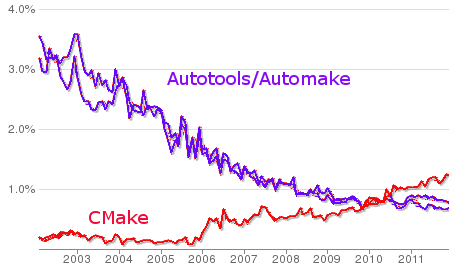
\includegraphics[width=0.9\textwidth,height=0.50\textheight]{compare_cmake_autotools_ohlo_color_transparent}
\end{center}
\begin{block}{\url{https://www.openhub.net/languages/compare}}
Language comparison of CMake to automake and
autoconf showing the percentage of developers commits that modify a
source file of the respective language (data from 2012).
\end{block}
\end{frame}

\begin{frame}
\frametitle{CMake/Autoconf/Gradle on Google Trend}
\begin{center}
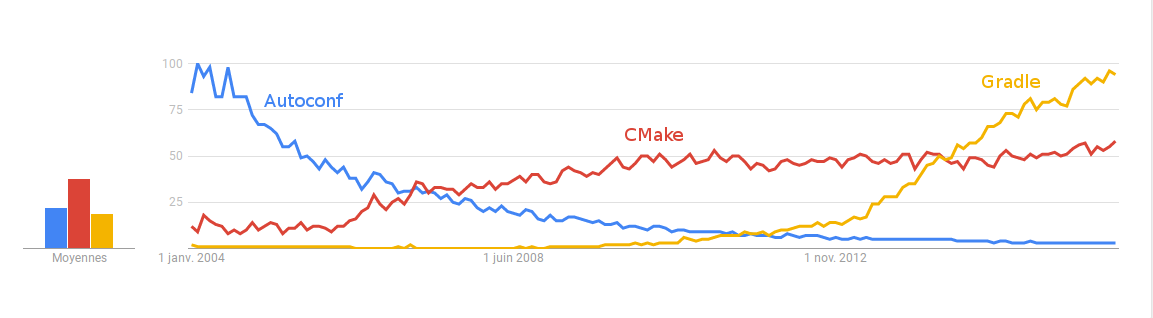
\includegraphics[width=1.0\textwidth,height=0.50\textheight]{CMakeAutoconfGradle-trend-2016}
\end{center}
\begin{block}{\url{https://www.google.com/trends}}
Scale is based on the average worldwide request traffic searching for CMake, Autoconf and Gradle in all years (2004--now).
\end{block}
\end{frame}

\section{Basic CMake usage}

\begin{frame}
\frametitle{A build system generator}
\begin{itemize}
\item CMake is a \emph{generator}: it generates \emph{native} build systems files (Makefile, Ninja, IDE project files [XCode, CodeBlocks, Eclipse CDT, Codelite, Visual Studio, Sublime Text\ldots], \ldots),
\item CMake scripting language (declarative) is used to describe the build,
\item The developer edits \fname{CMakeLists.txt}, invokes CMake but
      should \emph{never} edit the generated files,
\item CMake may be (automatically) re-invoked by the build system,
\item CMake has friends who may be very handy (CPack, CTest, CDash)
\end{itemize}
\end{frame}

\begin{frame}
\frametitle{The CMake workflow}
\begin{enumerate}
\onslide<2->{\item \emph{CMake time}: CMake is running \& processing \fname{CMakeLists.txt}}
\onslide<3->{\item \emph{Build time}: the build tool runs and invokes (at least) the compiler}
\onslide<4->{\item \emph{Install time}: the compiled binaries are installed

             i.e. from build area to an install location.
            }
\onslide<5->{\item \emph{CPack time}: CPack is running for building package}
\onslide<6->{\item \emph{Package Install time}: the package (from previous step) is installed}
\end{enumerate}
\onslide<1->{
\begin{alertblock}{When do things take place?}
CMake is a \emph{generator} which means it does not compile (i.e. build) the sources,
the underlying build tool (make, Ninja, XCode, Visual Studio\ldots) does.
\end{alertblock}
}
\end{frame}

\begin{frame}[label=cmakeworkflow]
\frametitle{The CMake workflow (pictured)}
\begin{tikzpicture}[
sbase/.style={      % The shape:
                    rectangle,
                    % The size:
                    minimum size=2mm,
                    minimum width=2.0cm,
                    minimum width=0.5cm,
                    % The border:
                    thick,
                    draw=black!50!black!50,
                    % 50% red and 50% black,
                    % and that mixed with 50% white
                    % The filling:
                    top color=white,
                    % a shading that is white at the top...
                    bottom color=red!80!black!20, % and something else at the bottom
                    % Font
                    font=\itshape\scriptsize}
                    ]
\tikzstyle{edited} = [sbase,
                      draw,
                      bottom color=green!80!black!20,
                      %opacity=.5,
                      %fill=green!20,
                      rounded corners]
\tikzstyle{generated} = [sbase,
                      draw,
                      %dashed,
                      bottom color=red!80!black!20,
                      %opacity=.5,
                      %fill=green!20,
                      rounded corners]
\tikzstyle{installed} = [sbase,
                      draw,
                      bottom color=blue!80!black!20,
                      %opacity=.5,
                      %fill=green!20,
                      rounded corners]
\tikzstyle{pkg} = [installed,
                  dashed,
                  general shadow={fill=blue!60!black!40,shadow scale=1.05,shadow xshift=+2pt,shadow yshift=-2pt}
                  ]
\onslide<1->{
\node[edited] (cmakelists) {\begin{tabular}{c}
                            CMakeLists.txt
                           \end{tabular}
                            };
\node[edited,below=1cm and 0cm of cmakelists.south] (sourcefiles)
                           {\begin{tabular}{c}
                            Source files
                           \end{tabular}
                           };
            }
\onslide<2->{
\node[generated,right=0cm and 1.5cm of cmakelists.east] (projectfiles)
                           {\begin{tabular}{c}
                            Project file(s),\\
                            Makefiles, \ldots
                           \end{tabular}
                           };
\node[generated,below right=2cm and 1.5cm of cmakelists.east] (gensourcefiles) {\begin{tabular}{c}
                            Generated \\
                            Sources files
                           \end{tabular}
                           };
}
\onslide<3->{
\node[generated,right=0cm and 1.5cm of projectfiles.east] (objectfiles)  {\begin{tabular}{c}
                             Object files
                             \end{tabular}
                            };
}
\onslide<5->{
\node[pkg, below left=1.7cm and 0cm of sourcefiles.south] (spackage)
                            {\begin{tabular}{c}
                              Source \\
                              package
                            \end{tabular}
                            };
}
\node[above right=0.5cm and 2.0cm of spackage.east] (legendL){};
\node[right=0cm and 2.3cm of legendL.east] (legendR){};
\onslide<5->{
\node[pkg, below right=-1.5cm and 7cm of spackage.east] (bpackage)
                            {\begin{tabular}{c}
                              Binary \\
                              package
                            \end{tabular}
                            };
}
\onslide<6->{
\node[installed, below=0.7cm and 0cm of bpackage.south] (ipackage)
                            {\begin{tabular}{c}
                              Installed \\
                              package
                            \end{tabular}
                            };

}
\onslide<4->{
\node[installed, above=0.7cm and 0cm of bpackage.north] (binstalled)
                            {\begin{tabular}{c}
                              Installed \\
                              files
                            \end{tabular}
                            };
}
\tikzstyle{cmaketime} = [-latex,thick,color=green]
\tikzstyle{buildtime} = [-latex,thick,color=red]
\tikzstyle{installtime} = [-latex,thick,color=black]
\tikzstyle{cpacktime} = [-latex,thick,color=blue]
\tikzstyle{packageinstalltime} = [-latex,thick,color=black,dashed]
\onslide<2->{
\draw [cmaketime]           ([yshift=0.0cm]legendL.south) -- ([yshift=0.0cm]legendR.south)  node[above=-2pt,midway,font=\tiny] {CMake time};
}
\onslide<3->{
\draw [buildtime]          ([yshift=-0.5cm]legendL.south) -- ([yshift=-0.5cm]legendR.south) node[above=-2pt,midway,font=\tiny] {Build time};
}
\onslide<4->{
\draw [installtime]        ([yshift=-1.0cm]legendL.south) -- ([yshift=-1.0cm]legendR.south) node[above=-2pt,midway,font=\tiny] {Install time};
}
\onslide<5->{
\draw [cpacktime]          ([yshift=-1.5cm]legendL.south) -- ([yshift=-1.5cm]legendR.south) node[above=-2pt,midway,font=\tiny] {CPack time};
}
\onslide<6->{
\draw [packageinstalltime] ([yshift=-2.0cm]legendL.south) -- ([yshift=-2.0cm]legendR.south) node[above=-2pt,midway,font=\tiny] {Package Install time};
}
\begin{pgfonlayer}{background}
\onslide<2->{
\draw [cmaketime] (cmakelists) -- (projectfiles);
\draw [cmaketime] (cmakelists) -- (gensourcefiles);
\draw [cmaketime] (sourcefiles) -- (gensourcefiles);
}
\onslide<5->{
\draw [cpacktime] (cmakelists) -- (spackage);
\draw [cpacktime] (sourcefiles) -- (spackage);
\draw [cpacktime] ([xshift=-0.2cm]binstalled.south) -- ([xshift=-0.2cm]bpackage.north);
}
\onslide<3->{
\draw [buildtime] (sourcefiles) -- (objectfiles);
\draw [buildtime] (gensourcefiles) -- (objectfiles);
\draw [buildtime] (projectfiles) -- (gensourcefiles);
}
\onslide<4->{
\draw [installtime] (objectfiles) -- (binstalled);
\draw [installtime] (gensourcefiles) -- (binstalled);
\draw [installtime] (sourcefiles) -- (binstalled);
}
\onslide<6->{
\draw [packageinstalltime] (bpackage.south) -- (ipackage.north);
}
\end{pgfonlayer}
\end{tikzpicture}
\end{frame}

\begin{frame}[fragile]
\frametitle{Building an executable}
\begin{lstlisting}[basicstyle=\scriptsize,caption=Building a simple program]
cmake_minimum_required (VERSION 3.0)
# This project use C source code
project (TotallyFree C)
set(CMAKE_C_STANDARD 99)
set(CMAKE_C_EXTENSIONS False)
# build executable using specified list of source files
add_executable(Acrolibre acrolibre.c)
\end{lstlisting}
CMake scripting language is [mostly] declarative.
It has \emph{commands} which are documented from within CMake:
{\tiny
\begin{verbatim}
 $ cmake --help-command-list | wc -l 
 117
 $ cmake --help-command add_executable
...
  add_executable
       Add an executable to the project using the specified source files.
\end{verbatim}
}
\end{frame}

\begin{frame}[fragile,allowframebreaks]
\frametitle{Builtin documentation}
\begin{Verbatim}[commandchars=\\\{\},fontsize=\tiny,numbers=left,frame=topline,label=CMake builtin doc for 'project' command]
  $ cmake --help-command project
project
-------

Set a name, version, and enable languages for the entire project.

 project(<PROJECT-NAME> [LANGUAGES] [<language-name>...])
 project(<PROJECT-NAME>
         [VERSION <major>[.<minor>[.<patch>[.<tweak>]]]]
         [LANGUAGES <language-name>...])

Sets the name of the project and stores the name in the
``PROJECT_NAME`` variable.
[...]
       Optionally you can specify which languages your project supports.
       Example languages are \textcolor{cmakeblue}{CXX} (i.e.  C++), \textcolor{cmakeblue}{C}, \textcolor{cmakeblue}{Fortran}, etc.  By \textcolor{cmakered}{default C} \textcolor{cmakered}{and CXX are enabled}.
       E.g.  if you do  not have a C++ compiler, you can disable the check  for it by  explicitly
       listing the languages  you want  to support, e.g.  C. By using the special language "\textcolor{cmakeblue}{NONE}"
       all checks for any language can be disabled.
\end{Verbatim}
Online doc : \url{https://cmake.org/documentation/}\\
Unix Manual: {\scriptsize \texttt{cmake-variables(7)}, \texttt{cmake-commands(7)}, \texttt{cmake-xxx(7)}, \ldots}\\
All doc generated using \href{http://www.sphinx-doc.org/en/stable/builders.html}{Sphinx},
QtHelp file as well:\\
\begin{small}
\begin{enumerate}
\item get QtHelp file from CMake: \url{https://cmake.org/cmake/help/v3.6/CMake.qch}

      and copy it to \texttt{CMake-tutorial/examples/}
\item use CMake.qhcp you may find in the source of this tutorial:

      \texttt{CMake-tutorial/examples/CMake.qhcp}
\item compile QtHelp collection file:

      \texttt{qcollectiongenerator CMake.qhcp -o CMake.qhc}
\item display it using Qt Assistant:

  \texttt{assistant -collectionFile CMake.qhc}
\end{enumerate}
\end{small}
\end{frame}

\defverbatim[colored]{\genmake}{
\begin{Verbatim}[commandchars=\\\{\},fontsize=\tiny,numbers=left,frame=topline,label=Building with make]
 $ ls totally-free
 acrolibre.c  CMakeLists.txt
 $ mkdir build
 $ cd build
 $ cmake ../totally-free
 -- The C compiler identification is GNU 4.6.2
 -- Check for working C compiler: /usr/bin/gcc
 -- Check for working C compiler: /usr/bin/gcc -- works
 ...
 $ \textcolor{cmakeblue}{make}
 ...
  [100%] Built target Acrolibre
 $ ./Acrolibre toulibre
\end{Verbatim}
 }

\defverbatim[colored]{\genninja}{
\begin{Verbatim}[commandchars=\\\{\},fontsize=\tiny,numbers=left,frame=topline,label=Building with ninja]
 $ ls totally-free
 acrolibre.c  CMakeLists.txt
 $ \textcolor{cmakered}{mkdir build-ninja}
 $ \textcolor{cmakered}{cd build-ninja}
 $ cmake \textcolor{cmakered}{-GNinja} ../totally-free
 -- The C compiler identification is GNU 4.6.2
 -- Check for working C compiler: /usr/bin/gcc
 -- Check for working C compiler: /usr/bin/gcc -- works
 ...
 $ \textcolor{cmakered}{ninja}
 ...
 [6/6] Linking C executable Acrodictlibre
 $ ./Acrolibre toulibre
\end{Verbatim}
}

\defverbatim[colored]{\gencrosswin}{
\begin{Verbatim}[commandchars=\\\{\},fontsize=\tiny,numbers=left,frame=topline,label=Building with cross-compiler]
 $ ls totally-free
 acrolibre.c  CMakeLists.txt
 $ \textcolor{cmakegreen}{mkdir build-win32}
 $ \textcolor{cmakegreen}{cd build-win32}
 $ cmake \textcolor{cmakegreen}{-DCMAKE_TOOLCHAIN_FILE=../totally-free/Toolchain-cross-linux.cmake} ../totally-free
 -- The C compiler identification is GNU 6.1.1
 -- Check for working C compiler: /usr/bin/i686-w64-mingw32-gcc
 ...
 $ \textcolor{cmakegreen}{make}
 ...
 [100%] Linking C executable Acrolibre\textcolor{cmakegreen}{.exe}
 [100%] Built target Acrolibre
 $ ./Acrolibre toulibre
\end{Verbatim}
}

\begin{frame}[fragile]
\frametitle{Generating \& building}
\only<3>{\textcolor{cmakegreen}{Cross-}}Building with CMake and \only<1,3>{\textcolor{cmakeblue}{make}}\only<2>{\textcolor{cmakered}{ninja}} is easy:
\begin{center}
\only<1>{\genmake}\only<2>{\genninja}\only<3>{\gencrosswin}
\end{center}
\onslide<1->{
\begin{alertblock}{Source tree vs Build tree}
Even the most simple project should never mix-up sources
with generated files. CMake supports \emph{out-of-source} build.
\end{alertblock}}
\end{frame}

\begin{frame}[fragile]
\frametitle{Always build out-of-source}
\begin{alertblock}{Out-of-source is better}
People are lazy (me too) and they think that because
building in source is possible and authorizes less typing
they can get away with it.
In-source build is a \emph{BAD} choice.
\end{alertblock}
Out-of-source build is \emph{always} better because:
\begin{enumerate}
\pause
\item Generated files are separated from manually edited ones

      (thus you don't have to clutter your favorite VCS ignore files).
\pause
\item You can have several build trees for the same source tree
\pause
\item This way it's always safe to completely delete the build tree
      in order to do a clean build
\end{enumerate}
\end{frame}

\begin{frame}[fragile]
\frametitle{Building program + autonomous library}
\onslide<2->{
\begin{block}{Conditional build}
We want to keep a version of our program that can be compiled
and run without the new Acrodict library \emph{and} the new version which
uses the library.
\end{block}}
We now have the following set of files in our source tree:
\begin{itemize}
\item \fname{acrolibre.c}, the main C program
\item \fname{acrodict.h}, the Acrodict library header
\item \fname{acrodict.c}, the Acrodict library source
\item \fname{CMakeLists.txt}, the soon to be updated CMake input file
\end{itemize}
\end{frame}

\begin{frame}[fragile]
\setlength{\columnsep}{0.8cm}
\vspace*{-0.5cm}
\begin{center}
The main program source
\end{center}
\begin{multicols}{2}
\begin{lstlisting}[basicstyle=\tiny,language=C,breaklines=true]
#include <stdlib.h>
#include <stdio.h>
#include <strings.h>
#ifdef USE_ACRODICT
#include "acrodict.h"
#endif
int main(int argc, char* argv[]) {

  const char * name;
#ifdef USE_ACRODICT
  const acroItem_t*  item;
#endif

  if (argc < 2) {
    fprintf(stderr,"%s: you need one argument\n",argv[0]);
    fprintf(stderr,"%s <name>\n",argv[0]);
    exit(EXIT_FAILURE);
  }
  name = argv[1];

#ifndef USE_ACRODICT
  if (strcasecmp(name,"toulibre")==0) {
    printf("Toulibre is a french organization promoting FLOSS.\n");
  }
#else
  item = acrodict_get(name);
  if (NULL!=item) {
    printf("%s: %s\n",item->name,item->description);
  } else if (item=acrodict_get_approx(name)) {
    printf("<%s> is unknown may be you mean:\n",name);
    printf("%s: %s\n",item->name,item->description);
  }
#endif
  else {
    printf("Sorry, I don't know: <%s>\n",name);
    return EXIT_FAILURE;
  }
  return EXIT_SUCCESS;
}
\end{lstlisting}
\end{multicols}
\end{frame}

\begin{frame}[fragile]
\setlength{\columnsep}{0.8cm}
\vspace*{-0.5cm}
\begin{center}
The library source
\end{center}
\begin{multicols}{2}
\begin{lstlisting}[basicstyle=\tiny,language=C,breaklines=true]
#ifndef ACRODICT_H
#define ACRODICT_H
typedef struct acroItem {
  char* name;
  char* description;
} acroItem_t;

const acroItem_t*
acrodict_get(const char* name);
#endif
\end{lstlisting}
\begin{lstlisting}[basicstyle=\tiny,language=C,breaklines=true]
#include <stdlib.h>
#include <string.h>
#include "acrodict.h"
static const acroItem_t acrodict[] = {
  {"Toulibre", "Toulibre is a french organization promoting FLOSS"},
  {"GNU", "GNU is Not Unix"},
  {"GPL", "GNU general Public License"},
  {"BSD", "Berkeley Software Distribution"},
  {"CULTe","Club des Utilisateurs de Logiciels libres et de gnu/linux de Toulouse et des environs"},
  {"Lea", "Lea-Linux: Linux entre ami(e)s"},
  {"RMLL","Rencontres Mondiales du Logiciel Libre"},
  {"FLOSS","Free Libre Open Source Software"},
  {"",""}};
const acroItem_t*
acrodict_get(const char* name) {
  int current =0;
  int found   =0;
  while ((strlen(acrodict[current].name)>0) && !found) {
    if (strcasecmp(name,acrodict[current].name)==0) {
      found=1;
    } else {
      current++;
    }
  }
  if (found) {
    return &(acrodict[current]);
  } else {
    return NULL;
  }
}
\end{lstlisting}
\end{multicols}
\end{frame}

\againframe{samplemakefile}

\begin{frame}[fragile]
\frametitle{Building a library}
\vspace*{-0.5cm}
\begin{lstlisting}[basicstyle=\tiny,caption=Building a simple program + shared library]
cmake_minimum_required (VERSION 3.0)
project (TotallyFree C) 
(*@\tikz[na] \coordinate(PdstC99);@*)set(CMAKE_C_STANDARD 99) 
set(CMAKE_C_EXTENSIONS False)
add_executable(Acrolibre acrolibre.c)
(*@\tikz[na] \coordinate(PdstVarDef);@*)set(LIBSRC acrodict.c acrodict.h) 
add_library(acrodict ${LIBSRC})(*@\tikz[na] \coordinate(PdstLibDef);@*)
add_executable(Acrodictlibre acrolibre.c)
(*@\tikz[na] \coordinate(PdstLinkOpt);@*)target_link_libraries(Acrodictlibre acrodict) (*@\label{linkline}@*)
(*@\tikz[na] \coordinate(PdstCompilOpt);@*)set_target_properties(Acrodictlibre PROPERTIES COMPILE_FLAGS "-DUSE_ACRODICT") (*@\label{propdef}@*)
\end{lstlisting}
\begin{itemize}
\item<1-> \tikz[na] \coordinate(PsrcC99);we precise that we want to compile with C99 flags
\item<2-> \tikz[na] \coordinate(PsrcVarDef);we define a variable and ask to build a library\tikz[na] \coordinate(PsrcLibDef);
\item<3-> \tikz[na] \coordinate(PsrcLinkOpt);we link an executable to our library %(line \ref{linkline})
\item<4-> \tikz[na] \coordinate(PsrcCompilOpt);we compile the source files of a particular target with specific compiler options
\end{itemize}

\begin{tikzpicture}[overlay]
  \only<1>{
    \path[->, red, thick] ($(PsrcC99)+(-0.5,0)$) edge[bend left] (PdstC99);
  }
  \only<2>{
    \path[->, red, thick] ($(PsrcVarDef)+(-0.5,0)$) edge[bend left] ($(PdstVarDef)+(0,-0.1)$);
  }
  \only<3>{
    \path[->, red, thick] ($(PsrcLinkOpt)+(-0.5,0)$) edge[bend left] ($(PdstLinkOpt)+(0,0)$);
  }
  \only<4>{
    \path[->, red, thick] ($(PsrcCompilOpt)+(-0.5,0)$) edge[bend left] ($(PdstCompilOpt)+(0,0)$);
  }
\end{tikzpicture}

\end{frame}

\begin{frame}[fragile,allowframebreaks]
\frametitle{Building a library - continued}

\begin{block}{And it builds...}
All in all CMake generates appropriate Unix makefiles which build
all this smoothly.
\end{block}
\begin{Verbatim}[fontsize=\tiny,numbers=left,frame=topline,label=CMake + Unix Makefile]
$ make
[ 33%] Building C object CMakeFiles/acrodict.dir/acrodict.c.o
Linking C shared library libacrodict.so
[ 33%] Built target acrodict
[ 66%] Building C object CMakeFiles/Acrodictlibre.dir/acrolibre.c.o
Linking C executable Acrodictlibre
[ 66%] Built target Acrodictlibre
[100%] Building C object CMakeFiles/Acrolibre.dir/acrolibre.c.o
Linking C executable Acrolibre
[100%] Built target Acrolibre
$ ls -F
Acrodictlibre*  CMakeCache.txt  cmake_install.cmake  Makefile
Acrolibre*      CMakeFiles/     libacrodict.so*
\end{Verbatim}

\begin{block}{And it works...}
We get the two different variants of our program, with varying capabilities.
\end{block}
\begin{multicols}{2}
\begin{Verbatim}[fontsize=\tiny,numbers=left]
$ ./Acrolibre toulibre
Toulibre is a french organization promoting FLOSS.
$ ./Acrolibre FLOSS
Sorry, I don't know: <FLOSS>
$ ./Acrodictlibre FLOSS
FLOSS: Free Libre Open Source Software
\end{Verbatim}
%$
\begin{Verbatim}[fontsize=\tiny,]
$ make help
The following are some of the valid targets
    for this Makefile:
... all (the default if no target is provided)
... clean
... depend
... Acrodictlibre
... Acrolibre
... acrodict
...
\end{Verbatim}
%$
Generated \fname{Makefile}s has several builtin targets besides the
expected ones:
\begin{itemize}
\item one per target (library or executable)
\item clean, all
\item more to come \ldots
\end{itemize}
\end{multicols}

\begin{alertblock}{And it is homogeneously done whatever the generator...}
  The obtained build system contains the same set of targets whatever the combination
  of generator and [cross-]compiler used: Makefile+gcc, Ninja+clang, XCode, Visual Studio, etc\ldots
\end{alertblock}
\end{frame}

\begin{frame}[fragile]
\frametitle{User controlled build option}
\begin{alertblock}{User controlled option}
Maybe our users don't want the acronym dictionary support.
We can use CMake \lstinline!OPTION! command.
\end{alertblock}
\begin{lstlisting}[basicstyle=\tiny,caption=User controlled build option]
cmake_minimum_required (VERSION 3.0)
# This project use C source code
project (TotallyFree C)
# Build option with default value to ON
option(WITH_ACRODICT "Include acronym dictionary support" ON)
set(BUILD_SHARED_LIBS true)
# build executable using specified list of source files
add_executable(Acrolibre acrolibre.c)
if (WITH_ACRODICT)
   set(LIBSRC acrodict.h acrodict.c)
   add_library(acrodict ${LIBSRC})
   add_executable(Acrodictlibre acrolibre.c)
   target_link_libraries(Acrodictlibre acrodict)
   set_target_properties(Acrodictlibre PROPERTIES COMPILE_FLAGS "-DUSE_ACRODICT")
endif(WITH_ACRODICT)
\end{lstlisting}
%$
\end{frame}


\begin{frame}[fragile,allowframebreaks]
  \frametitle{Too much keyboard, time to click?}

\begin{block}{CMake comes with severals tools}
  A matter of choice / taste:
  \vspace*{0.4cm}
\begin{itemize}
\item a command line: \fname{cmake}
\item a curses-based TUI: \fname{ccmake}
\item a Qt-based GUI: \fname{cmake-gui}
\end{itemize}
\end{block}

\begin{alertblock}{Calling convention}
All tools expect to be called with a single argument
which may be interpreted in 2 different ways.
\vspace*{0.4cm}
\begin{itemize}
\item path to the source tree, e.g.: \fname{cmake /path/to/source}
\item path to an \alert{existing} build tree, e.g.: \fname{cmake-gui .}
\end{itemize}
\end{alertblock}

\begin{center}
\fname{ccmake} : the curses-based TUI (demo)

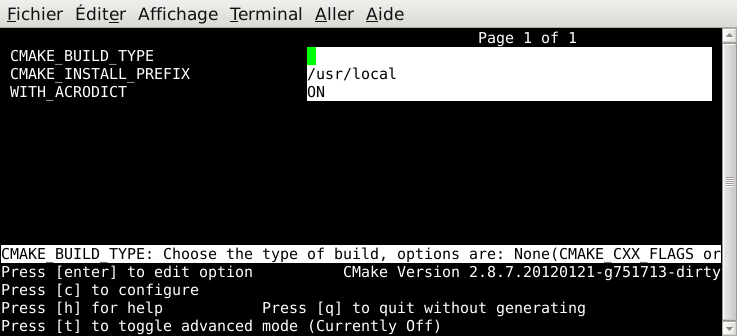
\includegraphics[width=0.8\textwidth]{ccmake-1}

Here we can choose to toggle the \lstinline!WITH_ACRODICT OPTION!.
\end{center}

\begin{center}
\fname{cmake-gui} : the Qt-based GUI (demo)

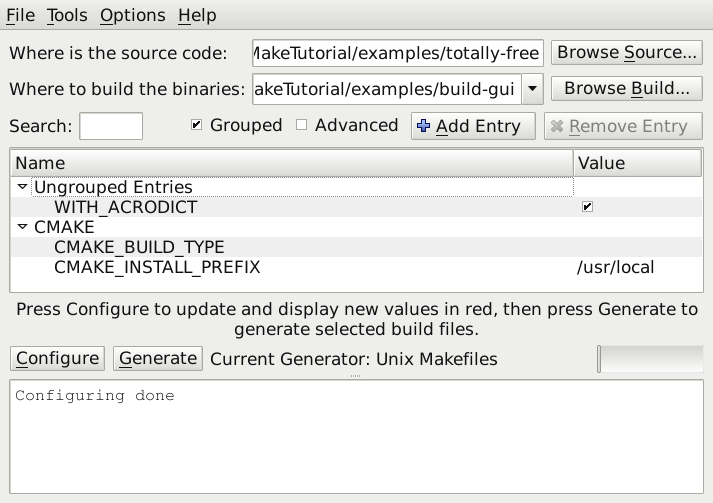
\includegraphics[width=0.7\textwidth]{cmake-gui-1}

Again, we can choose to toggle the \lstinline!WITH_ACRODICT OPTION!.
\end{center}
\end{frame}

\begin{frame}[fragile]
\frametitle{Remember CMake is a build \alert{generator}?}
The number of active generators depends on the platform
we are running on {Unix}, \textcolor{cmakered}{Apple},
\textcolor{cmakeblue}{Windows}:
\begin{multicols}{2}
\begin{Verbatim}[commandchars=\\\{\},fontsize=\scriptsize,numbers=left]
 \textcolor{cmakeblue}{Borland Makefiles}
 \textcolor{cmakeblue}{MSYS Makefiles}
 \textcolor{cmakeblue}{MinGW Makefiles}
 \textcolor{cmakeblue}{NMake Makefiles}
 \textcolor{cmakeblue}{NMake Makefiles JOM}
 Unix Makefiles
 \textcolor{cmakeblue}{Visual Studio 10}
 \textcolor{cmakeblue}{Visual Studio 10 IA64}
 \textcolor{cmakeblue}{Visual Studio 10 Win64}
 \textcolor{cmakeblue}{Visual Studio 11}
 \textcolor{cmakeblue}{Visual Studio 11 Win64}
 \textcolor{cmakeblue}{Visual Studio 6}
 \textcolor{cmakeblue}{Visual Studio 7}
 \textcolor{cmakeblue}{Visual Studio 7 .NET 2003}
 \textcolor{cmakeblue}{Visual Studio 8 2005}
 \textcolor{cmakeblue}{Visual Studio 8 2005 Win64}
 \textcolor{cmakeblue}{Visual Studio 9 2008}
 \textcolor{cmakeblue}{Visual Studio 9 2008 IA64}
 \textcolor{cmakeblue}{Visual Studio 9 2008 Win64}
 \textcolor{cmakeblue}{Watcom WMake}
 \textcolor{cmakeblue}{CodeBlocks - MinGW Makefiles}
 \textcolor{cmakeblue}{CodeBlocks - NMake Makefiles}
 CodeBlocks - Unix Makefiles
 \textcolor{cmakeblue}{Eclipse CDT4 - MinGW Makefiles}
 \textcolor{cmakeblue}{Eclipse CDT4 - NMake Makefiles}
 Eclipse CDT4 - Unix Makefiles
 KDevelop3
 KDevelop3 - Unix Makefiles
 \textcolor{cmakered}{XCode}
 Ni\textcolor{cmakeblue}{nj}\textcolor{cmakered}{a}
\end{Verbatim}

\end{multicols}
\end{frame}

\begin{frame}[fragile]
\frametitle{Equally simple on other platforms}
It is as easy for a Windows build, however
names for executables and libraries are computed
in a
\textcolor{cmakeblue}{platform}
\textcolor{cmakered}{specific}
\textcolor{cmakegreen}{way}.
\begin{center}
\begin{Verbatim}[commandchars=\\\{\},fontsize=\tiny,numbers=left,frame=topline,label=CMake + MinGW Makefile]
 $ ls totally-free
 acrodict.h acrodict.c acrolibre.c  CMakeLists.txt
 $ mkdir build-win32
 $ cd build-win32
 $ cmake -DCMAKE_TOOLCHAIN_FILE=../totally-free/Toolchain-cross-linux.cmake ../totally-free
 ...
 $ make
 Scanning dependencies of target acrodict
 \textcolor{cmakeblue}{[ 33%] Building C object CMakeFiles/acrodict.dir/acrodict.c.obj}
 \textcolor{cmakegreen}{Linking C shared library libacrodict.dll}
 \textcolor{cmakegreen}{Creating library file: libacrodict.dll.a}
 [ 33%] Built target acrodict
 Scanning dependencies of target Acrodictlibre
 \textcolor{cmakeblue}{[ 66%] Building C object CMakeFiles/Acrodictlibre.dir/acrolibre.c.obj}
 \textcolor{cmakered}{Linking C executable Acrodictlibre.exe}
 [ 66%] Built target Acrodictlibre
 Scanning dependencies of target Acrolibre
 \textcolor{cmakeblue}{[100%] Building C object CMakeFiles/Acrolibre.dir/acrolibre.c.obj}
 \textcolor{cmakered}{Linking C executable Acrolibre.exe}
 [100%] Built target Acrolibre
\end{Verbatim}
\end{center}
\end{frame}

\begin{frame}[fragile]
\frametitle{Installing things}
\begin{block}{Install}
Several parts or the software may need to be installed:
this is controlled by the CMake \lstinline!install! command.

\alert{Remember \fname{cmake --help-command install}!!}
\end{block}
\begin{lstlisting}[basicstyle=\tiny,caption=install command examples]
...
add_executable(Acrolibre acrolibre.c)
install(TARGETS Acrolibre DESTINATION bin)
if (WITH_ACRODICT)
  ...
  install(TARGETS Acrodictlibre acrodict
           RUNTIME DESTINATION bin
           LIBRARY DESTINATION lib
           ARCHIVE DESTINATION lib/static)
  install(FILES acrodict.h DESTINATION include)
endif(WITH_ACRODICT)
\end{lstlisting}
\end{frame}

\begin{frame}[fragile]
\frametitle{Controlling installation destination}
\begin{alertblock}{Use relative \lstinline!DESTINATION!}
One should always use relative installation \lstinline!DESTINATION!
unless you really want to use absolute path like \fname{/etc}.
\end{alertblock}
Then depending on when you install:
\begin{itemize}
\pause
\item At \textcolor{cmaketimec}{CMake-time} set \lstinline!CMAKE_INSTALL_PREFIX! value

     \begin{Verbatim}
   $ cmake --help-variable CMAKE_INSTALL_PREFIX
     \end{Verbatim}
\pause
\item At \textcolor{installtimec}{Install-time} use \fname{DESTDIR} mechanism (Unix Makefiles)

      \begin{Verbatim}
   $ make DESTDIR=/tmp/testinstall install
      \end{Verbatim}
\pause
\item At \textcolor{cpacktimec}{CPack-time}, CPack what? \ldots be patient.
\item At \textcolor{installtimec}{Package-install-time}, we will see that later
\end{itemize}
%\begin{Verbatim}[commandchars=\\\{\},fontsize=\tiny,numbers=left]
%\end{Verbatim}
\end{frame}

\againframe<6>{cmakeworkflow}

\begin{frame}[fragile]
\frametitle{Using CMake variables}
\begin{block}{CMake variables}
They are used by the user to simplify its \fname{CMakeLists.txt},
but CMake uses many (\textasciitilde 400+) of them to control/change its [default] behavior.
Try: \texttt{cmake --help-variable-list}.
\end{block}
\begin{block}{Inside a CMake script}
\lstinline!set(CMAKE_INSTALL_PREFIX /home/eric/testinstall)!
\begin{Verbatim}
$ cmake --help-command set
\end{Verbatim}
%$
\end{block}
\begin{block}{On the command line/TUI/GUI}
Remember that (besides options) each CMake tool takes a single argument
(source tree or \alert{existing} build tree)
\begin{Verbatim}[fontsize=\scriptsize]
$ cmake -DCMAKE_INSTALL_PREFIX=/home/eric/testinstall .
\end{Verbatim}
%$
\end{block}
\end{frame}

\begin{frame}[fragile]
\frametitle{The install target}
\begin{block}{Install target}
The \fname{install} target of the underlying build tool (in our case \fname{make})
appears in the generated build system as soon as some \lstinline!install! 
commands are used in the \fname{CMakeLists.txt}.
\end{block}
\begin{Verbatim}[commandchars=\\\{\},fontsize=\scriptsize,numbers=left]
$ make DESTDIR=/tmp/testinstall install
[ 33%] Built target acrodict
[ 66%] Built target Acrodictlibre
[100%] Built target Acrolibre
Install the project...
-- Install configuration: ""
-- Installing: /tmp/testinstall/bin/Acrolibre
-- Installing: /tmp/testinstall/bin/Acrodictlibre
-- Removed runtime path from "/tmp/testinstall/bin/Acrodictlibre"
-- Installing: /tmp/testinstall/lib/libacrodict.so
-- Installing: /tmp/testinstall/include/acrodict.h
$
\end{Verbatim}
\end{frame}

\begin{frame}[fragile]
\frametitle{Package the whole thing}
\vspace*{-0.4cm}
\begin{block}{CPack}
CPack is a CMake friend application (detailed later) which may be used to
easily package your software.
\end{block}
\vspace*{-0.7cm}
\begin{multicols}{2}
\begin{lstlisting}[basicstyle=\tiny,caption=add CPack support,]
...
endif(WITH_ACRODICT)
...
# Near the end of the CMakeLists.txt
# Chose your CPack generator
set(CPACK_GENERATOR "TGZ")
# Setup package version
set(CPACK_PACKAGE_VERSION_MAJOR 0)
set(CPACK_PACKAGE_VERSION_MINOR 1)
set(CPACK_PACKAGE_VERSION_PATCH 0)
# 'call' CPack
include(CPack)
\end{lstlisting}
\columnbreak
\begin{Verbatim}[commandchars=\\\{\},fontsize=\tiny]
$ make \textcolor{buildtimec}{package}
[ 33%] Built target acrodict
[ 66%] Built target Acrodictlibre
[100%] Built target Acrolibre
\textcolor{cpacktimec}{Run CPack packaging tool...}
CPack: Create package using TGZ
CPack: Install projects
CPack: - Run preinstall target for: TotallyFree
CPack: - Install project: TotallyFree
CPack: Create package
CPack: - package: <build-tree>/...
      TotallyFree-0.1.0-Linux.tar.gz generated.
$ tar ztvf TotallyFree-0.1.0-Linux.tar.gz
... TotallyFree-0.1.0-Linux/include/acrodict.h
... TotallyFree-0.1.0-Linux/bin/Acrolibre
... TotallyFree-0.1.0-Linux/bin/Acrodictlibre
... TotallyFree-0.1.0-Linux/lib/libacrodict.so
\end{Verbatim}
\end{multicols}
\end{frame}

\begin{frame}[fragile]
\frametitle{CPack the packaging friend}
\begin{block}{CPack is a standalone generator}
As we will see later on, CPack is standalone application,
which like CMake is a \emph{generator}.
\end{block}
\vspace*{-0.5cm}
\begin{multicols}{2}
\begin{Verbatim}[commandchars=\\\{\},fontsize=\tiny]
$ \textcolor{cpacktimec}{cpack -G ZIP}
CPack: Create package using ZIP
CPack: Install projects
CPack: - Run preinstall target for: TotallyFree
CPack: - Install project: TotallyFree
CPack: Create package
CPack: - package: <build-tree>/...
      TotallyFree-0.1.0-Linux.zip generated.
$ unzip -t TotallyFree-0.1.0-Linux.zip
Archive:  TotallyFree-0.1.0-Linux.zip
    testing: To.../include/acrodict.h   OK
    testing: To.../bin/Acrolibre   OK
    testing: To.../bin/Acrodictlibre   OK
    testing: To.../lib/libacrodict.so   OK
No errors detected in compressed
   data of TotallyFree-0.1.0-Linux.zip.
\end{Verbatim}
\columnbreak
\begin{Verbatim}[commandchars=\\\{\},fontsize=\tiny]
$ \textcolor{cpacktimec}{cpack -G RPM}
CPack: Create package using RPM
CPack: Install projects
CPack: - Run preinstall target for: TotallyFree
CPack: - Install project: TotallyFree
CPack: Create package
CPackRPM: Will use GENERATED spec file: <build-tree>/...
      _CPack_Packages/Linux/RPM/SPECS/totallyfree.spec
CPack: - package: <build-tree>/...
      TotallyFree-0.1.0-Linux.rpm generated.
$ rpm -qpl TotallyFree-0.1.0-Linux.rpm 
/usr
/usr/bin
/usr/bin/Acrodictlibre
/usr/bin/Acrolibre
/usr/include
/usr/include/acrodict.h
/usr/lib
/usr/lib/libacrodict.so
\end{Verbatim}
\end{multicols}
\end{frame}

\begin{frame}[fragile,allowframebreaks]
\frametitle{Didn't you mentioned testing?}
\vspace*{-0.4cm}
\begin{block}{CTest}
CTest is a CMake friend application (detailed later) which may be used to
easily test your software (if not cross-compiled though).
\end{block}
\vspace*{-0.7cm}
\begin{multicols}{2}
\begin{lstlisting}[escapechar={§},basicstyle=\tiny,caption=add CTest support]
...
endif(WITH_ACRODICT)
...
enable_testing()
add_test(toulibre-builtin
         Acrolibre "toulibre")
add_test(toulibre-dict
         Acrodictlibre "toulibre")
add_test(FLOSS-dict
         Acrodictlibre "FLOSS")
add_test(FLOSS-fail
         Acrolibre "FLOSS")
\end{lstlisting}
\columnbreak
\begin{Verbatim}[commandchars=\\\{\},fontsize=\tiny]
$ make \textcolor{buildtimec}{test}
Running tests...
Test project <buildtree-prefix>/build
    Start 1: toulibre-builtin
1/4 Test #1: toulibre-builtin ....   Passed  0.00 sec
    Start 2: toulibre-dict
2/4 Test #2: toulibre-dict........   Passed  0.00 sec
    Start 3: FLOSS-dict
3/4 Test #3: FLOSS-dict ..........   Passed  0.00 sec
    Start 4: FLOSS-fail
\textcolor{orange}{4/4 Test #4: FLOSS-fail ..........***Failed  0.00 sec}
75% tests passed, 1 tests failed out of 4
Total Test time (real) =   0.01 sec
The following tests FAILED:
	  4 - FLOSS-fail (Failed)
\end{Verbatim}
%$
\end{multicols}
\vspace*{-0.4cm}
\begin{block}{Tailor success rule}
CTest uses the return code in order to get success/failure status, but
one can tailor the success/fail rule.
\end{block}
\vspace*{-0.7cm}
\begin{multicols}{2}
\begin{lstlisting}[escapechar={§},basicstyle=\tiny,caption=add CTest support]
...
endif(WITH_ACRODICT)
...
enable_testing()
add_test(toulibre-builtin
         Acrolibre "toulibre")
add_test(toulibre-dict
         Acrodictlibre "toulibre")
add_test(FLOSS-dict
         Acrodictlibre "FLOSS")
add_test(FLOSS-fail
         Acrolibre "FLOSS")
set_tests_properties (FLOSS-fail
         PROPERTIES
         PASS_REGULAR_EXPRESSION
         "Sorry, I don't know:.*FLOSS")
\end{lstlisting}
\columnbreak
\begin{Verbatim}[commandchars=\\\{\},fontsize=\tiny]
$ make \textcolor{buildtimec}{test}
Running tests...
Test project <buildtree-prefix>/build
    Start 1: toulibre-builtin
1/4 Test #1: toulibre-builtin ....   Passed  0.00 sec
    Start 2: toulibre-dict
2/4 Test #2: toulibre-dict........   Passed  0.00 sec
    Start 3: FLOSS-dict
3/4 Test #3: FLOSS-dict ..........   Passed  0.00 sec
    Start 4: FLOSS-fail
4/4 Test #4: FLOSS-fail ..........   Passed  0.00 sec

100% tests passed, 0 tests failed out of 4

Total Test time (real) =   0.01 sec
\end{Verbatim}
%$
\end{multicols}
\end{frame}

\begin{frame}[fragile]
\frametitle{CTest the testing friend}
\begin{block}{CTest is a standalone generic test driver}
CTest is standalone application, which can run a set of \emph{test} programs.
\end{block}
\vspace*{-0.5cm}
\begin{multicols}{2}
\begin{Verbatim}[commandchars=\\\{\},fontsize=\tiny]
$ ctest -R toulibre-
Test project <build-tree>/build
    Start 1: toulibre-builtin
1/2 Test #1: toulibre-builtin .. Passed 0.00 sec
    Start 2: toulibre-dict
2/2 Test #2: toulibre-dict ..... Passed 0.00 sec

100% tests passed, 0 tests failed out of 2

Total Test time (real) =   0.01 sec
\end{Verbatim}
\columnbreak
\begin{Verbatim}[commandchars=\\\{\},fontsize=\tiny]
$ ctest -R FLOSS-fail -V
Test project <build-tree>
Constructing a list of tests
Done constructing a list of tests
Checking test dependency graph...
Checking test dependency graph end
test 4
    Start 4: FLOSS-fail
4: Test command: <build-tree>/Acrolibre "FLOSS"
4: Test timeout computed to be: 9.99988e+06
4: Sorry, I don't know: <FLOSS>
1/1 Test #4: FLOSS-fail ...........***Failed 0.00 sec

0% tests passed, 1 tests failed out of 1
Total Test time (real) =   0.00 sec

The following tests FAILED:
	  4 - FLOSS-fail (Failed)
Errors while running CTest
\end{Verbatim}
\end{multicols}
\end{frame}

\begin{frame}[fragile]
\frametitle{CDash the test results publishing}
\begin{block}{Dashboard}
CTest may help publishing the results of the tests
on a CDash dashboard (\url{http://www.cdash.org/}) 
for easing collective regression testing.
More on this later\ldots
\end{block}
%Example of an open-source project using CMake/CPack/CTest/CDash:
\begin{center}
{\scriptsize
\url{http://www.orfeo-toolbox.org/}--\url{http://dash.orfeo-toolbox.org/}
}

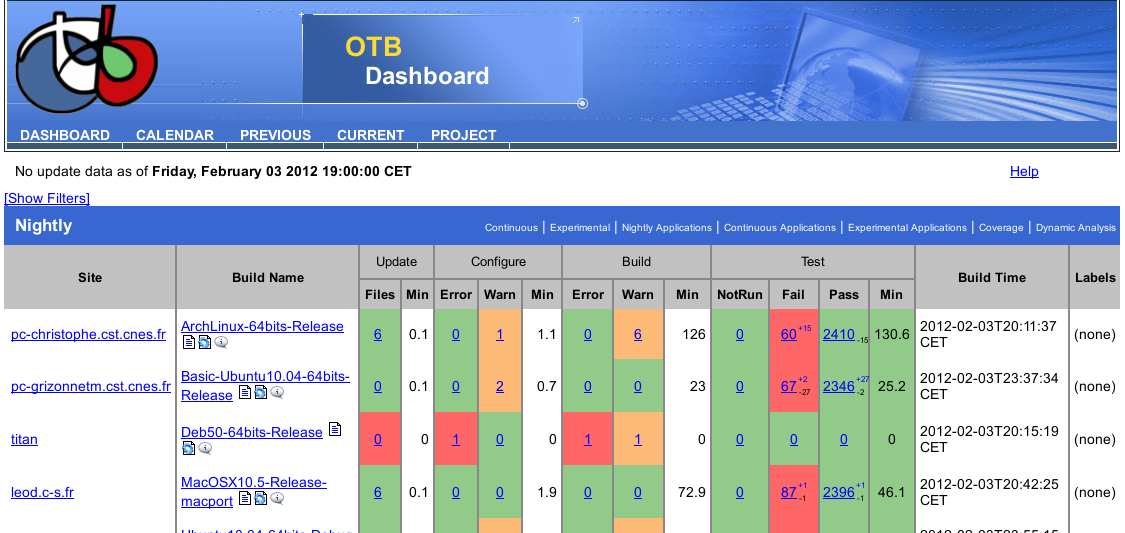
\includegraphics[width=0.7\textwidth]{OrfeoToolboxDashBoard}
\end{center}
\end{frame}


\begin{frame}[fragile]
\frametitle{Summary}
\begin{block}{CMake basics}
Using CMake basics we can already do a lot of things with minimal writing.
\end{block}
\begin{itemize}
\item Write simple build specification file: \fname{CMakeLists.txt}
\item Discover compilers (C, C++, Fortran)
\item Build executable and library (shared or static) in a cross-platform manner
\item Package the resulting binaries with CPack
\item Run systematic tests with CTest and publish them with CDash
\end{itemize}
\end{frame}

\begin{frame}[fragile]
\frametitle{Seeking more information or help}
There are several places you can go by yourself:
\begin{enumerate}
\item {\tiny(re-)}Read the documentation: \url{https://cmake.org/documentation}
\item Read the FAQ: \url{https://cmake.org/Wiki/CMake_FAQ}
\item Read the Wiki: \url{https://cmake.org/Wiki/CMake}
\item Ask on the Mailing List: \url{https://cmake.org/mailing-lists}
\item Browse the built-in help:

     \fname{man cmake-xxxx}\\
     \fname{cmake --help-xxxxx}\\
     \fname{assistant -collectionFile examples/CMake.qhc}
\end{enumerate}
\end{frame}

\section{Discovering environment specificities}
\subsection{Handling platform specificities}
\begin{frame}[fragile]
\frametitle{How to discover system}
\begin{block}{System/compiler specific variables}
Right after the \lstinline!project! command CMake has set up variables which can be used to tailor
the build in a platform specific way.
\end{block}
\lstset{basicstyle=\small}
\begin{itemize}
\item system specific
\begin{itemize}
\item \lstinline!WIN32! True on Windows systems, including Win64.
\item \lstinline!UNIX! True for UNIX and UNIX like operating systems.
\item \lstinline!APPLE! True if running on Mac OS X.
\item \lstinline!CYGWIN! True for Cygwin.
\item Have a look at \fname{cmake --system-information} output
\end{itemize}
\item compiler specific
\begin{itemize}
\item \lstinline!CMAKE_<LANG>_COMPILER_ID! A short string unique to the compiler vendor : Clang, GNU, MSVC, Cray, Absoft TI, XL\ldots
\end{itemize}
\end{itemize}
\lstset{basicstyle=\normalsize}
\end{frame}

\begin{frame}[fragile]
\frametitle{Handle system specific code}
Some functions like \lstinline[language=C]!strcasestr!
(lines \ref{strcasestr:l1} and \ref{strcasestr:l2}) may not be available
on all platforms.
\begin{lstlisting}[language=C,basicstyle=\tiny,xleftmargin=1cm,xrightmargin=1cm,caption=excerpt from acrodict.c]
const acroItem_t* acrodict_get_approx(const char* name) {
  int current =0;
  int found   =0;
#ifdef GUESS_NAME
  while ((strlen(acrodict[current].name)>0) && !found) {
    if ((strcasestr(name,acrodict[current].name)!=0) || (*@ \label{strcasestr:l1} @*)
        (strcasestr(acrodict[current].name,name)!=0)) { (*@ \label{strcasestr:l2} @*)
      found=1;
    } else {
      current++;
    }
  }
  if (found) {
    return &(acrodict[current]);
  } else
#endif
  {
    return NULL;
  }
}
\end{lstlisting}
\end{frame}

\begin{frame}[fragile]
\frametitle{Use system specific \lstinline!option!}
\begin{lstlisting}[basicstyle=\tiny]
# Build option with default value to ON
option(WITH_ACRODICT "Include acronym dictionary support" ON)
if(NOT WIN32)
  option(WITH_GUESS_NAME "Guess acronym name" ON) (*@ \label{no-win32-option} @*)
endif(NOT WIN32)
...
if (WITH_ACRODICT)
   # list of sources in our library
   set(LIBSRC acrodict.h acrodict.c)
   if (WITH_GUESS_NAME)
     set_source_files_properties(acrodict.c PROPERTIES COMPILE_FLAGS "-DGUESS_NAME") (*@ \label{source-specific-flags} @*)
   endif(WITH_GUESS_NAME)
   add_library(acrodict ${LIBSRC})
...
\end{lstlisting}
%$
Line \ref{no-win32-option} defines a CMake option, but not on \lstinline!WIN32! system.
Then on line \ref{source-specific-flags}, if the option is set then we pass a source specific compile flags.

\texttt{cmake --help-command set\_source\_files\_properties}
\end{frame}

\begin{frame}[fragile]
\frametitle{System specific in real life}
\begin{block}{Real [numeric] life project}
Real projects (i.e. not the toy of this tutorial) have many parts
of their \fname{CMakeLists.txt} which deal with system/compiler
specific option/feature.
\end{block}
\begin{itemize}
\item \href{http://musescore.org}{MuseScore}
\item \href{https://savannah.nongnu.org/projects/certi/}{CERTI},
{\scriptsize \url{http://git.savannah.gnu.org/cgit/certi.git/tree}}
\item \href{https://forge.onera.fr/projects/schedmcore}{SchedMCore},
{\scriptsize \url{https://svn.onera.fr/schedmcore/trunk/}}
\item \href{http://cmake.org}{CMake} (of course)
\item \href{http://llvm.org}{LLVM}, {\scriptsize \url{http://llvm.org/docs/CMake.html}}
\item many more \ldots
\end{itemize}
\end{frame}

\begin{frame}[fragile,allowframebreaks]
\frametitle{What about \fname{projectConfig.h} file?}
\begin{block}{Project config files}
Sometimes it's easier to test for features and then write a
configuration file (\fname{config.h}, \fname{project\_config.h}, \ldots).
The CMake way to do that is to:
\vspace*{0.4cm}
\begin{enumerate}
\item lookup system information using CMake variable, functions, macros (built-in or imported)
      then set various variables,
\item use the defined variable in order to write a template configuration
      header file
\item then use \lstinline!configure_file! in order to produce the actual
      config file from the template.
\end{enumerate}
\end{block}

\begin{lstlisting}[basicstyle=\tiny,caption=Excerpt from CERTI project's main \fname{CMakeLists.txt}]
# Load Checker macros
INCLUDE(CheckFunctionExists)

FIND_FILE(HAVE_STDINT_H NAMES stdint.h)
FIND_FILE(HAVE_SYS_SELECT_H NAMES select.h
  PATH_SUFFIXES sys)
INCLUDE(CheckIncludeFile)
CHECK_INCLUDE_FILE(time.h HAVE_TIME_H)
FIND_LIBRARY(RT_LIBRARY rt)
if(RT_LIBRARY)
  SET(CMAKE_REQUIRED_LIBRARIES ${CMAKE_REQUIRED_LIBRARIES} ${RT_LIBRARY})
endif(RT_LIBRARY)

CHECK_FUNCTION_EXISTS(clock_gettime HAVE_CLOCK_GETTIME)
CHECK_FUNCTION_EXISTS(clock_settime HAVE_CLOCK_SETTIME)
CHECK_FUNCTION_EXISTS(clock_getres HAVE_CLOCK_GETRES)
CHECK_FUNCTION_EXISTS(clock_nanosleep HAVE_CLOCK_NANOSLEEP)
IF (HAVE_CLOCK_GETTIME AND HAVE_CLOCK_SETTIME AND HAVE_CLOCK_GETRES)
    SET(HAVE_POSIX_CLOCK 1)
ENDIF (HAVE_CLOCK_GETTIME AND HAVE_CLOCK_SETTIME AND HAVE_CLOCK_GETRES)
...
CONFIGURE_FILE(${CMAKE_CURRENT_SOURCE_DIR}/config.h.cmake
               ${CMAKE_CURRENT_BINARY_DIR}/config.h)
\end{lstlisting}
\begin{Verbatim}[fontsize=\tiny,numbers=left,frame=topline,label=Excerpt from CERTI \fname{config.h.cmake}]
/* define if the compiler has numeric_limits<T> */
#cmakedefine HAVE_NUMERIC_LIMITS

/* Define to 1 if you have the <stdint.h> header file. */
#cmakedefine HAVE_STDINT_H 1

/* Define to 1 if you have the <stdlib.h> header file. */
#cmakedefine HAVE_STDLIB_H 1

/* Define to 1 if you have the <strings.h> header file. */
#cmakedefine HAVE_STRINGS_H 1
...
/* Name of package */
#cmakedefine PACKAGE "@PACKAGE_NAME@"

/* Define to the address where bug reports for this package should be sent. */
#cmakedefine PACKAGE_BUGREPORT "@PACKAGE_BUGREPORT@"

/* Define to the full name of this package. */
#cmakedefine PACKAGE_NAME "@PACKAGE_NAME@"

/* Define to the full name and version of this package. */
#cmakedefine PACKAGE_STRING "@PACKAGE_NAME@-@PACKAGE_VERSION@"
\end{Verbatim}

And you get something like:
\begin{Verbatim}[fontsize=\tiny,numbers=left,frame=topline,label=Excerpt from generated CERTI \fname{config.h}]
/* define if the compiler has numeric_limits<T> */
#define HAVE_NUMERIC_LIMITS

/* Define to 1 if you have the <stdint.h> header file. */
#define HAVE_STDINT_H 1

/* Define to 1 if you have the <stdlib.h> header file. */
#define HAVE_STDLIB_H 1

/* Define to 1 if you have the <strings.h> header file. */
#define HAVE_STRINGS_H 1
...
/* Name of package */
/* #undef PACKAGE */

/* Define to the address where bug reports for this package should be sent. */
#define PACKAGE_BUGREPORT "certi-devel@nongnu.org"

/* Define to the full name of this package. */
#define PACKAGE_NAME "CERTI"

/* Define to the full name and version of this package. */
/* #undef PACKAGE_STRING */
\end{Verbatim}
\end{frame}

\subsection{Working with external packages}

\begin{frame}[fragile,allowframebreaks]
\frametitle{The \lstinline!find_package! command}
\begin{block}{Finding external package}
Project may be using external libraries, programs, files etc\ldots
Those can be found using the \lstinline!find_package! command.
\end{block}
\begin{lstlisting}[basicstyle=\scriptsize,caption=using libxml2]
find_package(LibXml2)
if (LIBXML2_FOUND)
    add_definitions(-DHAVE_XML ${LIBXML2_DEFINITIONS})
    include_directories(${LIBXML2_INCLUDE_DIR})
else (LIBXML2_FOUND)
    set(LIBXML2_LIBRARIES "")
endif (LIBXML2_FOUND)
...
target_link_libraries(MyTarget ${LIBXML2_LIBRARIES})
\end{lstlisting}
%$
\begin{itemize}
\item Find modules usually define standard variables (for module XXX)
     \begin{enumerate}
     \item \fname{XXX\_FOUND}: Set to false, or undefined, if we haven't found, or don't want to use \fname{XXX}.
     \item \fname{XXX\_INCLUDE\_DIRS}: The final set of include directories listed in one variable for use by client code.
     \item \fname{XXX\_LIBRARIES}: The libraries to link against to use \fname{XXX}.
           These should include full paths.
     \item \fname{XXX\_DEFINITIONS}: Definitions to use when compiling code that uses \fname{XXX}.
     \item \fname{XXX\_EXECUTABLE}: File location of the \fname{XXX} tool's binary.
     \item \fname{XXX\_LIBRARY\_DIRS}: Optionally, the final set of library directories listed in one variable for use by client code.
     \end{enumerate}
\item See doc \fname{cmake --help-module FindLibXml2}
\item Many modules are provided by CMake (230 as of CMake 3.6.2)
\item Projects which are built with CMake usually provide a \emph{Project Config} file
      see doc: \url{https://cmake.org/cmake/help/git-master/manual/cmake-packages.7.html}
\item You may write your own:

      \url{https://cmake.org/Wiki/CMake:Module_Maintainers}
\item A module may provide not only CMake variables but new CMake macros
      (we will see that later with the \lstinline!MACRO!, \lstinline!FUNCTION!
       CMake language commands)
\end{itemize}
\end{frame}

\begin{frame}[fragile]
\frametitle{The other \lstinline!find_xxxx! commands}
\begin{block}{The \lstinline!find_xxx! command family}
\lstinline!find_package! is a \emph{high level} module finding mechanism
but there are lower-level CMake commands which may be used to write
find modules or anything else inside \fname{CMakeLists.txt}
\end{block}
\begin{itemize}
\item to find an executable program: \lstinline!find_program!
\item to find a library: \lstinline!find_library!
\item to find any kind of file: \lstinline!find_file!
\item to find a path where a file resides: \lstinline!find_path!
\end{itemize}
\end{frame}

\begin{frame}[fragile, allowframebreaks]
  \frametitle{\texttt{FindPrelude.cmake} example}

  The \texttt{FindPrelude.cmake} is part of the \emph{Prelude} synchronous language compiler made by ONERA:
  \url{https://forge.onera.fr/projects/Prelude}. This a source-to-source compiler which takes as input prelude file (\texttt{.plul}) and generates a bunch of C files which may be compiled in a dynamic library. The \texttt{FindPrelude.cmake} helps to automatize this task.

  \lstinputlisting[basicstyle=\tiny]{FindPrelude.cmake}
\end{frame}

\begin{frame}[fragile, allowframebreaks]
\frametitle{Advanced use of external package}
\begin{block}{Installed External package}
The previous examples suppose that you have the package you are
looking for on your host.
\vspace*{0.4cm}
\begin{itemize}
\item you did install the runtime libraries
\item you did install eventual developer libraries, headers and tools
\end{itemize}
\end{block}
\alert{What if the external packages:}
\begin{itemize}
\item are only available as source (tarball, VCS repositories, \ldots)
\item use a build system (autotools or CMake or \ldots)
\end{itemize}

\begin{alertblock}{\fname{ExternalProject\_Add}}
The \fname{ExternalProject.cmake} CMake module defines a high-level
macro which does just that:
\vspace*{0.5cm}
\begin{enumerate}
\item download/checkout source
\item update/patch
\item configure
\item build
\item install (and test)
\end{enumerate}
\begin{center}
\ldots an external project
\end{center}
\end{alertblock}
\begin{Verbatim}
$ cmake --help-module ExternalProject
\end{Verbatim}
%$
\end{frame}


\section{More CMake scripting}
\begin{frame}[fragile]
\frametitle{The different CMake ``modes''}
\begin{itemize}
\item Normal mode: the mode used when processing \fname{CMakeLists.txt}
\item Command mode: \fname{cmake -E <command>}, command line mode
      which offers basic commands in a portable way:

      \onslide<2->{\alert{works on all supported CMake platforms}. I.e. you don't want to rely
      on shell or native command interpreter capabilities.}
\item Process scripting mode: \fname{cmake -P <script>}, used to execute
      a CMake script which is not a CMakeLists.txt filename.

      \onslide<3->{\alert{Not all CMake commands are scriptable!!}}
\item Wizard mode: \fname{cmake -i}, interactive equivalent of the Normal mode.
\end{itemize}
\end{frame}

\begin{frame}[fragile]
\frametitle{Command mode}
\begin{Verbatim}[commandchars=\\\{\},fontsize=\tiny,numbers=left,frame=topline,label=list of command mode commands]
  $ cmake -E
CMake Error: cmake version 3.6.2
Usage: cmake -E <command> [arguments...]
Available commands: 
  chdir dir cmd [args...]   - run command in a given directory
  compare_files file1 file2 - check if file1 is same as file2
  copy <file>... destination  - copy files to destination (either file or directory)
  copy_directory <dir>... destination   - copy content of <dir>... directories to 'destination' directory
  copy_if_different <file>... destination  - copy files if it has changed
  echo [<string>...]        - displays arguments as text
  echo_append [<string>...] - displays arguments as text but no new line
  env [--unset=NAME]... [NAME=VALUE]... COMMAND [ARG]...
                            - run command in a modified environment
  environment               - display the current environment
  make_directory <dir>...   - create parent and <dir> directories
  md5sum <file>...          - create MD5 checksum of files
  remove [-f] <file>...     - remove the file(s), use -f to force it
  remove_directory dir      - remove a directory and its contents
  rename oldname newname    - rename a file or directory (on one volume)
  tar [cxt][vf][zjJ] file.tar [file/dir1 file/dir2 ...]
                            - create or extract a tar or zip archive
  sleep <number>...         - sleep for given number of seconds
  time command [args...]    - run command and return elapsed time
  touch file                - touch a file.
  touch_nocreate file       - touch a file but do not create it.
Available on UNIX only:
  create_symlink old new    - create a symbolic link new -> old
\end{Verbatim}
%$
\end{frame}

\begin{frame}[fragile]
\frametitle{CMake scripting}
\begin{block}{Overview of CMake language}
CMake is a declarative language which contains 90+ \emph{commands}.
It contains general purpose constructs:
\lstinline!set,unset!,
\lstinline!if,elseif,else,endif!,
\lstinline!foreach!,
\lstinline!while!, \lstinline!break!
\end{block}
Remember:
\begin{Verbatim}[fontsize=\tiny,numbers=left]
$ cmake --help-command-list
$ cmake --help-command <command-name>
$ cmake --help-command message
cmake version 2.8.7
  message
       Display a message to the user.
         message([STATUS|WARNING|AUTHOR_WARNING|FATAL_ERROR|SEND_ERROR]
                 "message to display" ...)
       The optional keyword determines the type of message:
         (none)         = Important information
         STATUS         = Incidental information
         WARNING        = CMake Warning, continue processing
         AUTHOR_WARNING = CMake Warning (dev), continue processing
         SEND_ERROR     = CMake Error, continue but skip generation
         FATAL_ERROR    = CMake Error, stop all processing
\end{Verbatim}
%$
\end{frame}

\begin{frame}[fragile]
\frametitle{Higher level commands as well}
\lstset{basicstyle=\scriptsize}
\begin{itemize}
\item file manipulation with \lstinline[basicstyle=\normalsize]!file! : \lstinline!READ, WRITE, APPEND!,
      \lstinline!RENAME, REMOVE, MAKE_DIRECTORY!
      
\item advanced files operations: \lstinline!GLOB, GLOB_RECURSE! file name in a path,
      \lstinline!DOWNLOAD, UPLOAD!
\item working with path: \lstinline[basicstyle=\normalsize]!file!\lstinline!(TO_CMAKE_PATH /TO_NATIVE_PATH ...)!, \lstinline[basicstyle=\normalsize]!get_filename_component!
\item execute an external process (with stdout, stderr and return code retrieval): \lstinline[basicstyle=\normalsize]!execute_process!
\item builtin list manipulation command: \lstinline[basicstyle=\normalsize]!list! with sub-commands
      \lstinline!LENGTH, GET, APPEND!,
      \lstinline!FIND, APPEND, INSERT!,
      \lstinline!REMOVE_ITEM, REMOVE_AT, REMOVE_DUPLICATES!
      \lstinline!REVERSE, SORT!
\item string manipulation: \lstinline[basicstyle=\normalsize]!string!, upper/lower case conversion, length, comparison,
      substring, regular expression match, \ldots
\end{itemize}
\lstset{basicstyle=\normalsize}
\end{frame}

\begin{frame}[fragile,allowframebreaks]
\frametitle{Portable script for building CMake}
As an example of what can be done with pure CMake script
(script mode) here is a script for building the CMake package
using a previously installed CMake.
\lstinputlisting[basicstyle=\tiny,numbers=left,breaklines=true]{examples/CMake-autobuild-v2.cmake}

\end{frame}

\begin{frame}[fragile]
  \frametitle{Portable script for building ROSACE Case Study}
Another example taken from the ``\emph{ROSACE Open Source Case Study}'' may be found here
see \href{https://svn.onera.fr/schedmcore/branches/ROSACE_CaseStudy/prelude_implementations/instructions/ROSACE-CaseStudy-auto.cmake}{ROSACE-CaseStudy-auto.cmake}

The script:
\begin{itemize}
\item Download or checkout \href{https://cavale.enseeiht.fr/redmine/projects/lustrec}{Lustre} compiler and build it
\item Download or checkout \href{https://forge.onera.fr/projects/prelude}{Prelude} compiler and build it
\item Download or checkout \href{http://sites.onera.fr/schedmcore/}{SchedMCore} toolsuit and build it
\item Checkout the \href{http://sites.onera.fr/schedmcore/ROSACE}{ROSACE Case Study} and build it using the previously built tools.
\end{itemize}
\end{frame}

\begin{frame}[fragile]
\frametitle{Build specific commands}
\begin{itemize}
\item create executable or library: \lstinline!add_executable!, \lstinline!add_library!
\item add compiler/linker definitions/options: \lstinline!add_definition!, \lstinline!include_directories!,
      \lstinline!target_link_libraries!
\item powerful installation specification: \lstinline!install!
\item probing command: \lstinline!try_compile!, \lstinline!try_run!
\item fine control of various properties:
      \lstinline!set_target_properties!,
      \lstinline!set_source_files_properties!,
      \lstinline!set_directory_properties!,
      \lstinline!set_tests_properties!: \alert{300+} different properties may be used.
\end{itemize}
\begin{Verbatim}
$ cmake --help-property-list
$ cmake --help-property COMPILE_FLAGS
\end{Verbatim}
\end{frame}

\subsection{Custom commands}
\begin{frame}[fragile]
\frametitle{What are CMake targets?}
\begin{block}{CMake target}
Many times in the documentation you may read about CMake \emph{target}.
A target is something that CMake should build (i.e. generate something
enabling the building of the \emph{target}).

A CMake target has \alert{dependencies} and \alert{properties}.
\end{block}
\begin{enumerate}
\item Executables are targets: \lstinline!add_executable!
\item Libraries are targets: \lstinline!add_library!
\item There exist some builtin targets: \fname{install}, \fname{clean}, \fname{package}, \ldots
\item You may create custom targets: \lstinline!add_custom_target!
\end{enumerate}
\end{frame}

\begin{frame}[fragile,allowframebreaks]
\frametitle{Target dependencies and properties}
A CMake target has \alert{dependencies} and \alert{properties}.
\begin{block}{Dependencies}
Most of the time, source dependencies are computed from target specifications
using CMake builtin dependency scanner (C, C++, Fortran)
whereas library dependencies
are inferred via \lstinline!target_link_libraries! specification.
\end{block}
If this is not enough then one can use \lstinline!add_dependencies!,
or some properties.
\begin{block}{Properties}
Properties may be attached to either \emph{target} or \emph{source file}
(or even \emph{test}).
They may be used to tailor the prefix or suffix to be used for libraries,
compile flags, link flags, linker language, shared libraries version,
\ldots
\end{block}
\vspace*{-0.3cm}
see : \lstinline!set_target_properties! or \lstinline!set_source_files_properties!
\vspace*{-0.3cm}
\begin{alertblock}{Sources vs Targets}
Properties set to a target like \lstinline!COMPILE_FLAGS! are used
for all sources of the concerned target. Properties set to a source
are used for the source file itself (which may be involved in several targets).
\end{alertblock}
\end{frame}

\begin{frame}[fragile]
\frametitle{Custom targets and commands}
\begin{block}{Custom}
Custom targets and custom commands are a way to create a \emph{target}
which may be used to execute arbitrary commands at \alert{Build-time}.
\vspace*{0.4cm}
\begin{itemize}
\item for target  : \lstinline!add_custom_target!
\item for command : \lstinline!add_custom_command!, in order to add some
custom build step to another (existing) target.
\end{itemize}
\end{block}
This is usually for: generating source files (Flex, Bison) or
other files derived from source like embedded documentation (Doxygen), \ldots
\end{frame}

\subsection{Generated files}
\begin{frame}[fragile]
\frametitle{Generated files}
\begin{block}{List all the sources}
CMake advocates to specify all the source files explicitly
(i.e. do not use \lstinline!file(GLOB ...)!)
This is the only way to keep robust dependencies.
Moreover you usually already need to do that when using a VCS
(CVS, Subversion, Git, hg,\ldots).
\end{block}
However some files may be generated during the build (using \lstinline!add_custom_xxx!),
in which case you must tell CMake that they are \lstinline!GENERATED! files
using:

\begin{lstlisting}[basicstyle=\scriptsize]
set_source_files_properties(${SOME_GENERATED_FILES}
                            PROPERTIES GENERATED TRUE)
\end{lstlisting}
%$
\end{frame}

\againframe<6>{cmakeworkflow}

\begin{frame}[fragile,allowframebreaks]
\frametitle{Example}
\begin{lstlisting}[basicstyle=\tiny,numbers=left]
### Handle Source generation for task file parser
include_directories(${CMAKE_CURRENT_SOURCE_DIR})
find_package(LexYacc)
set(YACC_SRC               ${CMAKE_CURRENT_SOURCE_DIR}/lsmc_taskfile_syntax.yy)
set(YACC_OUT_PREFIX        ${CMAKE_CURRENT_BINARY_DIR}/y.tab)
set(YACC_WANTED_OUT_PREFIX ${CMAKE_CURRENT_BINARY_DIR}/lsmc_taskfile_syntax)
set(LEX_SRC               ${CMAKE_CURRENT_SOURCE_DIR}/lsmc_taskfile_tokens.ll)
set(LEX_OUT_PREFIX        ${CMAKE_CURRENT_BINARY_DIR}/lsmc_taskfile_tokens_yy)
set(LEX_WANTED_OUT_PREFIX ${CMAKE_CURRENT_BINARY_DIR}/lsmc_taskfile_tokens)

#Exec Lex
add_custom_command(
   OUTPUT  ${LEX_WANTED_OUT_PREFIX}.c
   COMMAND ${LEX_PROGRAM} ARGS -l -o${LEX_WANTED_OUT_PREFIX}.c ${LEX_SRC}
   DEPENDS ${LEX_SRC}
   )
set(GENERATED_SRCS ${GENERATED_SRCS} ${LEX_WANTED_OUT_PREFIX}.c)
#Exec Yacc
add_custom_command(
   OUTPUT  ${YACC_WANTED_OUT_PREFIX}.c ${YACC_WANTED_OUT_PREFIX}.h
   COMMAND ${YACC_PROGRAM} ARGS ${YACC_COMPAT_ARG} -d ${YACC_SRC}
   COMMAND ${CMAKE_COMMAND} -E copy ${YACC_OUT_PREFIX}.h  ${YACC_WANTED_OUT_PREFIX}.h
   COMMAND ${CMAKE_COMMAND} -E copy ${YACC_OUT_PREFIX}.c  ${YACC_WANTED_OUT_PREFIX}.c
   DEPENDS ${YACC_SRC}
   )
set(GENERATED_SRCS ${GENERATED_SRCS}
    ${YACC_WANTED_OUT_PREFIX}.c ${YACC_WANTED_OUT_PREFIX}.h)
# Tell CMake that some file are generated
set_source_files_properties(${GENERATED_SRCS} PROPERTIES GENERATED TRUE)

# Inhibit compiler warning for LEX/YACC generated files
# Note that the inhibition is COMPILER dependent ...
# GNU CC specific warning stop
if (CMAKE_COMPILER_IS_GNUCC)
   message(STATUS "INHIBIT Compiler warning for LEX/YACC generated files")
   SET_SOURCE_FILES_PROPERTIES(${YACC_WANTED_OUT_PREFIX}.c ${YACC_WANTED_OUT_PREFIX}.h
                                   PROPERTIES COMPILE_FLAGS "-w")

   SET_SOURCE_FILES_PROPERTIES(${LEX_WANTED_OUT_PREFIX}.c
                                   PROPERTIES COMPILE_FLAGS "-w")
endif(CMAKE_COMPILER_IS_GNUCC)
...
set(LSCHED_SRC
    lsmc_dependency.c  lsmc_core.c  lsmc_utils.c
    lsmc_time.c lsmc_taskfile_parser.c
    ${GENERATED_SRCS})
add_library(lsmc ${LSCHED_SRC})
\end{lstlisting}
\end{frame}

\section{Advanced CMake usage}
\subsection{Cross-compiling with CMake}
\begin{frame}[fragile]
\frametitle{Cross-compiling}
\begin{block}{Definition: Cross-compiling}
Cross-compiling is when the \emph{host} system,
\textsl{the one the compiler is running on},
is not the same as the \emph{target} system,
\textsl{the one the compiled program will be running on}.
\end{block}
CMake can handle cross-compiling using a \emph{Toolchain} description file,
see \url{https://cmake.org/Wiki/CMake_Cross_Compiling}.
\begin{Verbatim}[fontsize=\tiny,numbers=left]
mkdir build-win32
cd build-win32
cmake -DCMAKE_TOOLCHAIN_FILE=../totally-free/Toolchain-cross-mingw32-linux.cmake ../totally-free/
\end{Verbatim}
% $
\begin{center}
{\Large
\alert{Demo}
}
\end{center}

\end{frame}

\begin{frame}[fragile]
  \frametitle{Linux to Windows Toolchain example}
  \lstinputlisting[basicstyle=\tiny,numbers=left]{examples/totally-free/Toolchain-cross-linux.cmake}
\end{frame}

\subsection{Export your project}
\begin{frame}
\frametitle{Exporting/Import your project}

\begin{block}{Export/Import to/from others}
CMake can help a project using CMake as a build system to
export/import targets to/from another project using CMake
as a build system.
\end{block}

No more time for that today sorry, see:

\url{https://cmake.org/cmake/help/latest/manual/cmake-packages.7.html\#creating-packages}
\end{frame}

\part{CPack}
%\addcontentsline{toc}{part}{Part II: CPack}
\progressbaroptions{
  % headline=sections,
  imagename=figures/CPack-cube-3D-opened-small.png,
  titlepage=normal,
  frametitle=picture-section
}

\section{CPack: Packaging made easy}
\begin{frame}
\frametitle{Introduction}
\begin{block}{A Package \textbf{generator}}
In the same way that CMake \emph{generates} build files, CPack
\emph{generates} package files.
\end{block}

\begin{multicols}{2}
\begin{itemize}
\item Archive generators [ZIP,TGZ,\ldots] (All platforms)
\item DEB, RPM (Linux)
\item Cygwin Source or Binary (Windows/Cygwin)
\item NSIS (Windows, Linux)
\item DragNDrop, Bundle, OSXX11 (Mac OS)
\end{itemize}
\columnbreak

\includegraphics[width=5cm]{figures/CPack-logo-3D-opened-v2} \\
\end{multicols}
\end{frame}

\section{CPack with CMake}

\againframe<6>{cmakeworkflow}

\begin{frame}
\frametitle{The CPack application}
\begin{block}{CPack standalone}
CPack is a standalone application whose behavior is
driven by a configuration file e.g. \fname{CPackConfig.cmake}.
This file is a CMake language script which defines
\lstinline!CPACK_XXXX! variables:

the config parameters of the CPack run.
\end{block}
\begin{block}{CPack with CMake}
When CPack is used to package a project built with CPack,
then the CPack configuration is usually generated by CMake by
including \fname{CPack.cmake} in the main \fname{CMakeLists.txt}:

\lstinline!include(CPack)!
\end{block}
\end{frame}

\begin{frame}[fragile]
\frametitle{CPack variables in \fname{CMakeLists.txt}}
When used with CMake, one writes something like this in \fname{CMakeLists.txt}:
\begin{lstlisting}[basicstyle=\scriptsize,numbers=left]
set(CPACK_GENERATOR "TGZ")
if (WIN32)
   list(APPEND CPACK_GENERATOR "NSIS")
elseif (APPLE)
   list(APPEND CPACK_GENERATOR "Bundle")
endif(WIN32)
set(CPACK_SOURCE_GENERATOR "ZIP;TGZ")
set(CPACK_PACKAGE_VERSION_MAJOR 0)
set(CPACK_PACKAGE_VERSION_MINOR 1)
set(CPACK_PACKAGE_VERSION_PATCH 0)
include(CPack)
\end{lstlisting}
This will create \fname{CPackSourceConfig.cmake} and \fname{CPackConfig.cmake}
in the build tree and will bring you the \emph{\fname{package}} and \emph{\fname{package\_source}}
built-in targets.
\end{frame}

\begin{frame}[fragile, allowframebreaks]
\frametitle{A CPack config file}
A CPack config file looks like this one:
\begin{lstlisting}[basicstyle=\scriptsize,numbers=left,breaklines=true]
# This file will be configured to contain variables for CPack.
# These variables should be set in the CMake list file of the
# project before CPack module is included.
...
SET(CPACK_BINARY_BUNDLE "")
SET(CPACK_BINARY_CYGWIN "")
SET(CPACK_BINARY_DEB "")
...
SET(CPACK_BINARY_ZIP "")
SET(CPACK_CMAKE_GENERATOR "Unix Makefiles")
SET(CPACK_GENERATOR "TGZ")
SET(CPACK_INSTALL_CMAKE_PROJECTS "/home/erk/erkit/CMakeTutorial/examples/build;TotallyFree;ALL;/")
SET(CPACK_INSTALL_PREFIX "/usr/local")
SET(CPACK_MODULE_PATH "")
SET(CPACK_NSIS_DISPLAY_NAME "TotallyFree 0.1.0")
SET(CPACK_NSIS_INSTALLER_ICON_CODE "")
SET(CPACK_NSIS_INSTALL_ROOT "$PROGRAMFILES")
SET(CPACK_NSIS_PACKAGE_NAME "TotallyFree 0.1.0")
SET(CPACK_OUTPUT_CONFIG_FILE "/home/erk/erkit/CMakeTutorial/examples/build/CPackConfig.cmake")
SET(CPACK_PACKAGE_DEFAULT_LOCATION "/")
SET(CPACK_PACKAGE_DESCRIPTION_FILE "/home/erk/CMake/cmake-Verk-HEAD/share/cmake-2.8/Templates/CPack.GenericDescription.txt")
SET(CPACK_PACKAGE_DESCRIPTION_SUMMARY "TotallyFree built using CMake")
SET(CPACK_PACKAGE_FILE_NAME "TotallyFree-0.1.0-Linux")
SET(CPACK_PACKAGE_INSTALL_DIRECTORY "TotallyFree 0.1.0")
SET(CPACK_PACKAGE_INSTALL_REGISTRY_KEY "TotallyFree 0.1.0")
SET(CPACK_PACKAGE_NAME "TotallyFree")
SET(CPACK_PACKAGE_RELOCATABLE "true")
SET(CPACK_PACKAGE_VENDOR "Humanity")
SET(CPACK_PACKAGE_VERSION "0.1.0")
SET(CPACK_RESOURCE_FILE_LICENSE "/home/erk/CMake/cmake-Verk-HEAD/share/cmake-2.8/Templates/CPack.GenericLicense.txt")
SET(CPACK_RESOURCE_FILE_README "/home/erk/CMake/cmake-Verk-HEAD/share/cmake-2.8/Templates/CPack.GenericDescription.txt")
SET(CPACK_RESOURCE_FILE_WELCOME "/home/erk/CMake/cmake-Verk-HEAD/share/cmake-2.8/Templates/CPack.GenericWelcome.txt")
SET(CPACK_SET_DESTDIR "OFF")
SET(CPACK_SOURCE_CYGWIN "")
SET(CPACK_SOURCE_GENERATOR "TGZ;TBZ2;TZ")
SET(CPACK_SOURCE_OUTPUT_CONFIG_FILE "/home/erk/erkit/CMakeTutorial/examples/build/CPackSourceConfig.cmake")
SET(CPACK_SOURCE_TBZ2 "ON")
SET(CPACK_SOURCE_TGZ "ON")
SET(CPACK_SOURCE_TZ "ON")
SET(CPACK_SOURCE_ZIP "OFF")
SET(CPACK_SYSTEM_NAME "Linux")
SET(CPACK_TOPLEVEL_TAG "Linux")
\end{lstlisting}
%$
\end{frame}

\begin{frame}[fragile, allowframebreaks]
\frametitle{CPack running steps}
For a CMake enabled project one can run CPack in two ways:
\begin{enumerate}
\item use the build tool to run targets: \fname{package} or \fname{package\_source}
\item invoke CPack manually from within the \emph{build tree} e.g.:

      \fname{\$ cpack -G RPM}
\end{enumerate}
The CPack documentation is currently found on the Wiki or
on the CPack specific modules:
\begin{itemize}
\item \url{https://cmake.org/Wiki/CMake:CPackPackageGenerators}
\item \url{https://cmake.org/Wiki/CMake:Component_Install_With_CPack}
\item \fname{cpack --help-module CPackXXX} with CPack, CPackComponent, CPackRPM, CPackDEB, CPackIFW, CPackWIX, \ldots
\end{itemize}

Whichever way you call it, the CPack steps are:
\begin{enumerate}
\item cpack command starts and parses arguments etc\ldots
\item it reads \fname{CPackConfig.cmake} (usually found in the build tree)
      or the file given as an argument to \fname{--config} command line option.
\item it iterates over the generators list found in \fname{CPACK\_GENERATOR}
      (or from \fname{-G} command line option). For each generator:
      \begin{enumerate}
      \item (re)sets \fname{CPACK\_GENERATOR} to the one currently being iterated over
      \item includes the \fname{CPACK\_PROJECT\_CONFIG\_FILE}
      \item installs the project into a CPack private location (using \fname{DESTDIR})
      \item calls the generator and produces the package(s) for that generator
      \end{enumerate}
\end{enumerate}

\begin{Verbatim}[commandchars=\\\{\},fontsize=\scriptsize,numbers=left,frame=topline,label=cpack command line example]
$ cpack -G "TGZ;RPM"
\textcolor{blue}{CPack: Create package using TGZ}
CPack: Install projects
CPack: - Run preinstall target for: TotallyFree
CPack: - Install project: TotallyFree
CPack: Create package
CPack: - package: <...>/build/\textcolor{blue}{TotallyFree-0.1.0-Linux.tar.gz} generated.
\textcolor{blue}{CPack: Create package using RPM}
CPack: Install projects
CPack: - Run preinstall target for: TotallyFree
CPack: - Install project: TotallyFree
CPack: Create package
{\tiny CPackRPM: Will use GENERATED spec file: <...>/build/_CPack_Packages/Linux/RPM/SPECS/totallyfree.spec}
CPack: - package: <...>/build/\textcolor{blue}{TotallyFree-0.1.0-Linux.rpm} generated.
$
\end{Verbatim}
% $
\begin{Verbatim}[commandchars=\\\{\},fontsize=\scriptsize,numbers=left,frame=topline,label=make package example]
$ make package
[ 33%] Built target acrodict
[ 66%] Built target Acrodictlibre
[100%] Built target Acrolibre
Run CPack packaging tool...
CPack: Create package using TGZ
CPack: Install projects
CPack: - Run preinstall target for: TotallyFree
CPack: - Install project: TotallyFree
CPack: Create package
CPack: - package: <...>/build/TotallyFree-0.1.0-Linux.tar.gz generated.
\end{Verbatim}
%$
\begin{alertblock}{Rebuild project}
 In the \fname{make package} case CMake is checking that the project does not need a rebuild.
\end{alertblock}

\begin{Verbatim}[commandchars=\\\{\},fontsize=\scriptsize,numbers=left,frame=topline,label=make package\_source example]
$ make package_source
make package_source 
Run CPack packaging tool for source...
CPack: Create package using TGZ
CPack: Install projects
CPack: - Install directory: <...>/totally-free
CPack: Create package
CPack: - package: <...>/build/TotallyFree-0.1.0-Source.tar.gz generated.
CPack: Create package using TBZ2
CPack: Install projects
CPack: - Install directory: <...>/totally-free
CPack: Create package
CPack: - package: <...>/build/TotallyFree-0.1.0-Source.tar.bz2 generated.
CPack: Create package using TZ
CPack: Install projects
CPack: - Install directory: <...>/totally-free
CPack: Create package
CPack: - package: <...>/build/TotallyFree-0.1.0-Source.tar.Z generated.
\end{Verbatim}
%$
\end{frame}

\begin{frame}[label=cpackworkflow]
\frametitle{The CPack workflow (pictured)}
\begin{tikzpicture}[
sbase/.style={      % The shape:
                    rectangle,
                    % The size:
                    minimum size=2mm,
                    minimum width=2.0cm,
                    minimum width=0.5cm,
                    % The border:
                    thick,
                    draw=black!50!black!50,
                    % 50% red and 50% black,
                    % and that mixed with 50% white
                    % The filling:
                    top color=white,
                    % a shading that is white at the top...
                    bottom color=red!80!black!20, % and something else at the bottom
                    % Font
                    font=\itshape\scriptsize}
                    ]
\tikzstyle{edited} = [sbase,
                      draw,
                      bottom color=green!80!black!20,
                      %opacity=.5,
                      %fill=green!20,
                      rounded corners]
\tikzstyle{generated} = [sbase,
                      draw,
                      %dashed,
                      bottom color=red!80!black!20,
                      %opacity=.5,
                      %fill=green!20,
                      rounded corners]
\tikzstyle{installed} = [sbase,
                      draw,
                      bottom color=blue!80!black!20,
                      %opacity=.5,
                      %fill=green!20,
                      rounded corners]
\tikzstyle{pkg} = [installed,
                  dashed,
                  general shadow={fill=blue!60!black!40,shadow scale=1.05,shadow xshift=+2pt,shadow yshift=-2pt}
                  ]
\tikzstyle{boitearrondie} = [draw,
                             dashed,
                             opacity=.5,
                             fill=blue!20,
                             rounded corners]
\onslide<1->{
\node[edited] (cmakelists) {\begin{tabular}{c}
                            CMakeLists.txt
                           \end{tabular}
                            };
\node[edited,below=1cm and 0cm of cmakelists.south] (sourcefiles)
                           {\begin{tabular}{c}
                            Source files
                           \end{tabular}
                           };
            }
\onslide<4->{
\node[generated,right=0cm and 1.6cm of cmakelists.east] (cpackconf)
                           {\begin{tabular}{c}
                            CPackConfig.cmake
                           \end{tabular}
                           };
\node[generated,below=2.7cm and 0.0cm of cpackconf.south] (cpacksconf)
                           {\begin{tabular}{c}
                            CPackSourceConfig.cmake
                           \end{tabular}
                           };
            }
\node[below=1cm and -0.2cm of sourcefiles.south west] (legendL){};
\node[right=0cm and 2.3cm of legendL.east] (legendR){};
\onslide<5->{
\node[pkg, below=0.7cm and 0cm of cpacksconf.south] (spackage)
                            {\begin{tabular}{c}
                              Source \\
                              package
                            \end{tabular}
                            };
}

\onslide<7->{
\node[pkg, below=1.2cm and 0cm of cpackconf.south] (bpackage)
                            {\begin{tabular}{c}
                              Binary \\
                              package
                            \end{tabular}
                            };
           }
\onslide<8->{
\node[installed, right=0.0cm and 4.0cm of bpackage.west] (ipackage)
                            {\begin{tabular}{c}
                              Installed \\
                              package
                            \end{tabular}
                            };

            }
\begin{pgfonlayer}{background}
\onslide<6->{
\node[installed, below right=0.1cm and 0.1cm of cpackconf.south] (binstalled)
                            {\tiny
                             \begin{tabular}{c}
                             CPack\\
                             Installed files
                            \end{tabular}
                            };
            }
\end{pgfonlayer}
\tikzstyle{cmaketime} = [-latex,thick,color=green]
\tikzstyle{buildtime} = [-latex,thick,color=red]
\tikzstyle{installtime} = [-latex,thick,color=black,postaction={draw,red,dash pattern=on 4pt off 3pt,dash phase=4pt,thick,color=blue}]
\tikzstyle{cpacktime} = [-latex,thick,color=blue]
\tikzstyle{packageinstalltime} = [-latex,thick,color=black,dashed]
\onslide<3->{
\draw [cmaketime]           ([yshift=0.0cm]legendL.south) -- ([yshift=0.0cm]legendR.south)  node[above=-2pt,midway,font=\tiny] {CMake time};
\draw [buildtime]          ([yshift=-0.5cm]legendL.south) -- ([yshift=-0.5cm]legendR.south) node[above=-2pt,midway,font=\tiny] {Build time};
\draw [installtime]        ([yshift=-1.0cm]legendL.south) -- ([yshift=-1.0cm]legendR.south) node[above=-2pt,midway,font=\tiny] {Install time (from CPack)};
\draw [cpacktime]          ([yshift=-1.5cm]legendL.south) -- ([yshift=-1.5cm]legendR.south) node[above=-2pt,midway,font=\tiny] {CPack time};
\draw [packageinstalltime] ([yshift=-2.0cm]legendL.south) -- ([yshift=-2.0cm]legendR.south) node[above=-2pt,midway,font=\tiny] {Package Install time};
}

\begin{pgfonlayer}{background2}
\onslide<2->{
\draw[boitearrondie,top color=blue,bottom color=green,middle color=red] ([xshift=-0.2cm,yshift=0.2cm]cmakelists.north west) rectangle ([xshift=0.3cm,yshift=-0.2cm]sourcefiles.south east);
\pgftext[top,at={\pgfpointadd{\pgfpoint{0.0cm}{-0.4cm}}{\pgfpointanchor{cmakelists}{south}}},rotate=20]{\scriptsize Source Tree};
}
\onslide<3->{
\draw[boitearrondie,top color=blue,bottom color=green,middle color=red] ([xshift=-0.6cm,yshift=0.2cm]cpackconf.north west) rectangle ([xshift=1.4cm,yshift=-0.2cm]spackage.south east);
\pgftext[top,at={\pgfpointadd{\pgfpoint{-0.4cm}{0.8cm}}{\pgfpointanchor{bpackage}{west}}},rotate=40] {\scriptsize Build Tree};
\node (btree) {};
}
\end{pgfonlayer}

\begin{pgfonlayer}{background}
\onslide<4->{
\draw [cmaketime] (cmakelists) -- (cpackconf);
\draw [cmaketime] (cmakelists) -- (cpacksconf);
}
\onslide<5->{
\draw [cpacktime] ([yshift=0.2cm]sourcefiles.south) -- (spackage);
\draw [cpacktime] (cpacksconf) -- (spackage);
}
\onslide<7->{
\draw [cpacktime] ([xshift=-0.2cm]binstalled.south) -- ([xshift=0.2cm]bpackage.north);
\draw [cpacktime] (cpackconf) -- (bpackage);
}
\onslide<6->{
\draw [installtime] ([xshift=-1.4cm]binstalled.west) -- (binstalled);
}
\onslide<8->{
\draw [packageinstalltime] (bpackage.east) -- (ipackage.west);
}
\end{pgfonlayer}
\end{tikzpicture}
\end{frame}

\begin{frame}
\frametitle{Source vs Binary Generators}
\alert{CPack does not really distinguish ``source'' from ``binaries''!!}
\begin{block}{CPack source package}
The CPack configuration file is: \fname{CPackSourceConfig.cmake}.
The CPack source generator is essentially packaging directories with
install, exclude and include rules.
\end{block}
\begin{block}{CPack binary package}
The CPack configuration file is: \fname{CPackConfig.cmake}.
Moreover CPack knows that a project is built with CMake and
inherits many properties from the install rules found in
the project.
\end{block}

\end{frame}

\section{Various package generators}
\begin{frame}
\frametitle{Archive Generators}
\begin{block}{A family of generators}
The archive generators is a family of generators which is supported
on all CMake supported platforms through \fname{libarchive}:
\url{http://code.google.com/p/libarchive/}.
\end{block}
\begin{itemize}
\item[STGZ] Self extracting Tar GZip compression
\item[TBZ2] Tar BZip2 compression
\item[TGZ]  Tar GZip compression
\item[TZ]   Tar Compress compression
\item[TXZ]  Tar XZ compression
\item[7Z]   7-zip archive
\item[ZIP]  Zip archive
\end{itemize}
\end{frame}

\begin{frame}[allowframebreaks]
\frametitle{Linux-friendly generators}
\begin{itemize}
\item Tar-kind archive generators
\item Binary RPM: only needs \fname{rpmbuild} to work.
\item Binary DEB: works on any Linux distros.
\item IFW: Qt Installer framework
\end{itemize}
\begin{block}{CPack vs native tools}
One could argue ``why use CPack for building .deb or .rpm''.
The primary target of CPack RPM and DEB generators are people who are NOT
professional packagers.
Those people can get a clean package without too much effort and get
a better package than a bare TAR archive.
\end{block}
\begin{alertblock}{No official packaging replacement}
Those generators are \alert{no replacement} for official packaging tools.
\end{alertblock}
\end{frame}

\begin{frame}
\frametitle{Windows-friendly generators}
\begin{itemize}
\item Zip archive generator
\item NullSoft System Installer generator: \url{http://nsis.sourceforge.net/}

      Supports component installation, produces nice GUI installer.
\item WiX installer: \url{http://wixtoolset.org/}

  Windows Installer XML which produces MSI.
\item IFW: Qt Installer framework
\item Cygwin: Binary and Source generators.
\end{itemize}
\end{frame}

\begin{frame}
\frametitle{Mac OS-friendly generators}
\begin{multicols}{2}
\begin{itemize}
\item Tar-kind archive generators
\item DragNDrop
\item PackageMaker
\item Bundle
\item OSXX11
\item may be Qt IFW as well...
\end{itemize}
\end{multicols}
\begin{alertblock}{Don't ask me}
I'm not a Mac OS user and I don't know them.
Go and read the CPack doc or ask on the ML.
\url{https://cmake.org/mailing-lists/}
\end{alertblock}
\end{frame}

\begin{frame}[fragile,allowframebreaks]
\frametitle{Packaging Components}
\vspace*{-0.7cm}
\begin{block}{CMake+CPack installation components?}
Sometimes you want to split the installer into \emph{components}.
\end{block}
\vspace*{-0.7cm}
\begin{enumerate}
\item Use \fname{COMPONENT} argument in your install rules
      (in the CMakeLists.txt),
\item Add some more [CPack] information about how to group
      components,
\item Choose a component-aware CPack generator
\item Choose the behavior (1 package file per component, 1 package file
      per group, etc\ldots)
\item Possibly specify generator specific behavior in \fname{CPACK\_PROJECT\_CONFIG\_FILE}
\item Run CPack.
\end{enumerate}
\begin{center}
\alert{demo with ComponentExample}
\end{center}

More detailed documentation here:

{\scriptsize \url{https://cmake.org/Wiki/CMake:Component_Install_With_CPack}}
\begin{alertblock}{Component aware generator}
\begin{itemize}
\item Not all generators do support components

      (i.e. they are \fname{MONOLITHIC})
\item Some produce a single package file containing all components.

      (e.g. NSIS, WiX, Qt IFW)
\item Others produce several package files containing one or several components.

      (e.g. ArchiveGenerator, RPM, DEB)
\end{itemize}
\end{alertblock}
\end{frame}


% \section{CPack and cross-compiling}
\part{CTest and CDash}
%\addcontentsline{toc}{part}{Part III: CTest and CDash}

\progressbaroptions{
  % headline=sections,
  imagename=figures/cdash-logo.png,
  titlepage=normal,
  frametitle=picture-section
}
\section{Systematic Testing}
% \begin{frame}
% \frametitle{Systematic testing with CTest}

% \end{frame}
\section{CTest submission to CDash}
% \begin{frame}
% \frametitle{Systematic testing with CTest}

% \end{frame}

\begin{frame}
\frametitle{More to come on CTest/CDash}
\begin{block}{Sorry...out of time!!}
CMake and its friends are so much fun and powerful that
I ran out of time to reach a detailed presentation of
CTest/CDash, stay tuned for next time\ldots
\end{block}
In the meantime:
\begin{itemize}
\item Go there: \url{http://www.cdash.org}
\item Open your own (free) Dashboard: \url{http://my.cdash.org/}
\end{itemize}
\end{frame}

\section{References}
\begin{frame}[allowframebreaks]
\frametitle{References}
\nocite{CMakeBookv6,CDash:Home,CMake:Home,CMake:Wiki,KDE:Techbase:CMake,CMake:Documentation,LLVM:CMakePrimer}
\bibliographystyle{plain}
\bibliography{CMake-biblio}
\end{frame}

\end{document}



% LocalWords:  CMake
